\renewcommand{\prevlecture}{1 }
\renewcommand{\thislecture}{2 }
\renewcommand{\nextlecture}{3 }

%
% Cover page
%

\title[PHYS 201 / Lecture \thislecture]
{
  PHYS 201 / Lecture \thislecture \\
    {\it Electric flux; Gauss' law}\\
}

\author[C.Andreopoulos] {
  Professor Costas Andreopoulos\inst{1,2}, {\it FHEA}
}
\institute[Liverpool/STFC-RAL] {
   \inst{1} University of Liverpool, Department of Physics\\
   \vspace{0.1cm}
   \inst{2} U.K. Research \& Innovation (UKRI), Science \& Technology Facilities Council,\\
            Rutherford Appleton Laboratory, Particle Physics Department\\
   \vspace{0.5cm}
   {\it {\color{magenta} Lectures delivered at the University of Liverpool, 2020-21}}\\
   \vspace{0.2cm}
}
\date{\today}

\titlegraphic{
  
\includegraphics[height=25px]{./images/logo/liverpool.png}
  \hspace{3px}
  
\includegraphics[height=30px]{./images/logo/ral.png}
}


\begin{frame}[plain]
  \titlepage
\end{frame}

% ------------------------------------------------------------------------------
% ------------------------------------------------------------------------------

%
% Revision of previous lecture
%

\renewcommand{\lecturesummarytitle}{Revision }
\renewcommand{\summarizedlecture}{1 }

%
%
%

\begin{frame}{Lecture \summarizedlecture - \lecturesummarytitle}

\begin{itemize}
{\small
\item {\bf Electric charge}
  \begin{itemize}
  {\small
    \item The source of electric phenomena
    \item An intrinsic property of matter
    \item Comes in two varieties (positive and negative)
    \item An algebraic quantity (+q + (-q) = 0)
    \item It is quantised
    \item It is conserved (globally and locally)
    \item SI unit: Coulomb (C) [= 1 A $\cdot$ 1 s]
  }
  \end{itemize}

\vspace{0.2cm}

\item {\bf Coulomb's law}
  \begin{itemize}
  {\small
     \item Describes the force between two point charges
     \item The force $\vec{F}_{12}$ exerted on test charge 1 by charge 2 is:
     \begin{equation*}
       \vec{F}_{12} = \frac{1}{4\pi\epsilon_0} \frac{q_1 q_2}{|\vec{r}_{1}-\vec{r}_{2}|^{2}} \hat{r}_{12}
       \;\;\;
       or
       \;\;\;
       \vec{F}_{12} = \frac{1}{4\pi\epsilon_0} \frac{q_1 q_2}{|\vec{r}_{1}-\vec{r}_{2}|^{3}} (\vec{r}_{1}-\vec{r}_{2})
     \end{equation*}
  }
  \end{itemize}

}
\end{itemize}

\end{frame}


%
%
%

\begin{frame}{Lecture \summarizedlecture - \lecturesummarytitle (cont'd)}

\begin{itemize}
{\small

\item {\bf Superposition principle}
  \begin{itemize}
  {\small
     \item Allows the calculation of the total force on a charge Q
           from an array of other charges $q_1$, $q_2$, ..., $q_n$
      \begin{equation*}
       \vec{F}_{Q} = \sum_{i=1}^{n} \frac{1}{4\pi\epsilon_0}
          \frac{Q q_i}{|\vec{r}_{Q}-\vec{r}_{q_{i}}|^{3}} (\vec{r}_{Q}-\vec{r}_{q_{i}})
       \end{equation*}
     \item Total force is the vector sum of forces.
     \item Not a logical necessity: An experimental fact!
  }
  \end{itemize}

\vspace{0.2cm}

\item {\bf Continuous distributions of charge}
  \begin{itemize}
  {\small
    \item Made the leap from discrete to continuous charge distributions described by a charge density
    \item Reformulated Coulomb's law for continuous charge distributions
     \begin{equation*}
        \vec{F}_{Q} = \frac{Q}{4\pi\epsilon_0} \int_{\tau}
           d\tau^{\prime} \frac{\rho({\pvec{r}'})}{|\vec{r}-\pvec{r}'|^{3}} (\vec{r}-\pvec{r}')
     \end{equation*}
  }
  \end{itemize}

}
\end{itemize}

\end{frame}

%
%
%

\begin{frame}{Lecture \summarizedlecture - \lecturesummarytitle (cont'd)}

\begin{itemize}
{\small

\item {\bf Electric field}
  \begin{itemize}
  {\small
     \item A more fundamental way to think about electric forces in terms of a field that permeates space.
     \item Defined the electric field $\vec{E}$
           as the force exerted on a test charge Q, placed in position $\vec{r}$, per unit charge.
      \begin{equation*}
        \vec{E}(\vec{r}) = \frac{\vec{F}_Q(\vec{r})}{Q}
      \end{equation*}
  }
  \end{itemize}

\item {\bf Visualizing the electric field - field lines}
  \begin{itemize}
  {\small
     \item Field direction indicated by the direction of field lines
     \item Field strength indicated by the density of field lines
     \item Force tangential to field lines
     \item Field lines start from positive charges and end on negative ones:
           Positive charges are "sources", negative charges are "sinks"
     \item Field lines can not cross
  }
  \end{itemize}
}
\end{itemize}

\end{frame}


%
% Plan for this lecture
%

\begin{frame}{Plan for Lecture \thislecture}

\begin{itemize}
{\small
\item {\bf Electric flux}
  \begin{itemize}
  {\scriptsize
     \item The "flow" of an electric field (i.e. the number of electric field lines) through a surface.
  }
  \end{itemize}

\item {\bf Gauss' law}
  \begin{itemize}
  {\scriptsize
     \item Relates the flux through a closed surface with the net charge contained in it.
     \item Our first Maxwell equation! Will study both its `differential' and `integral' forms.
  }
  \end{itemize}
}
\end{itemize}

\end{frame}

% ------------------------------------------------------------------------------
% ------------------------------------------------------------------------------

%
%
%

\begin{frame}{Electric flux}

The flux $\Phi_E$ of the electric field $\vec{E}$ through a surface S is the {\em number of field lines}
flowing through S.
\begin{itemize}
 \item
   The number of field lines, and thus $\Phi_E$ is proportional to $|\vec{E}|$ and, obviously, proportional to S.
 \item
   The flux decreases if the surface is not perpendicular to the field, and becomes zero when the surface
   is parallel to the field.
\end{itemize}

\begin{columns}
  \begin{column}{0.33\textwidth}
   \begin{center}
    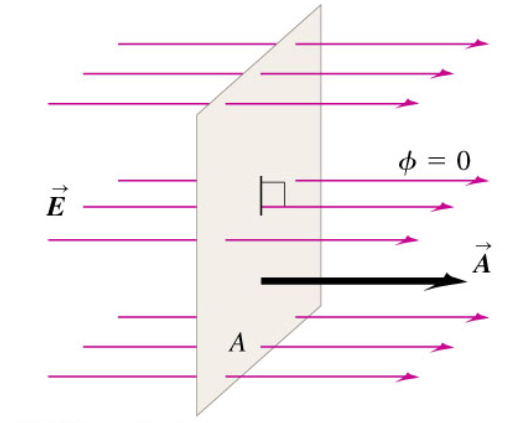
\includegraphics[width=0.98\textwidth]{./images/schematics/electric_flux_surface_perpendicular.png}\\
   \end{center}
  \end{column}
  \begin{column}{0.33\textwidth}
   \begin{center}
    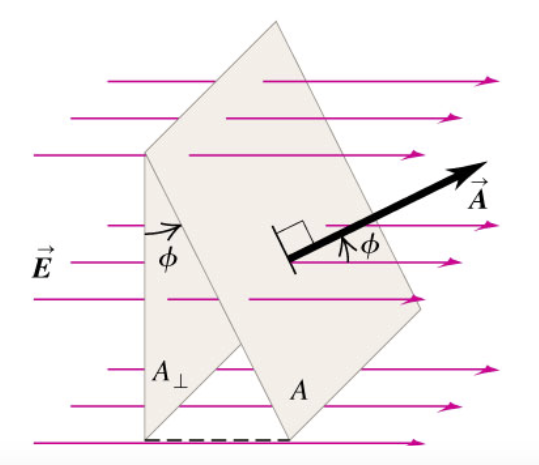
\includegraphics[width=0.98\textwidth]{./images/schematics/electric_flux_surface_angle.png}\\
   \end{center}
  \end{column}
  \begin{column}{0.33\textwidth}
   \begin{center}
    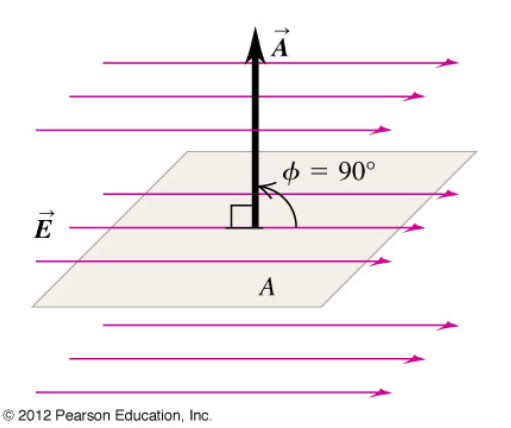
\includegraphics[width=0.98\textwidth]{./images/schematics/electric_flux_surface_parallel.png}\\
   \end{center}
  \end{column}
\end{columns}

\begin{center}
  We can write the electric flux as $\Phi_E = |\vec{E}| \; S \; cos\theta$.
\end{center}

\end{frame}


%
%
%

\begin{frame}{Electric flux}

\begin{columns}
  \begin{column}{0.33\textwidth}
   \begin{center}
    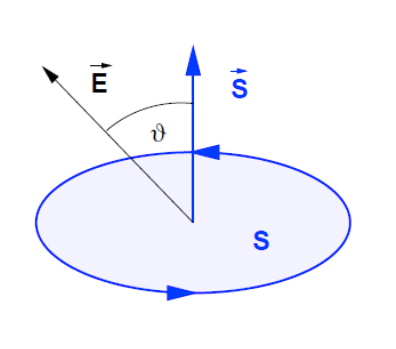
\includegraphics[width=0.98\textwidth]{./images/schematics/electric_flux_surface.png}\\
    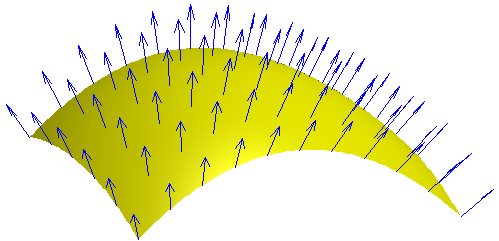
\includegraphics[width=0.98\textwidth]{./images/schematics/surface_normal.png}\\
    {\scriptsize
     Note that if the surface is closed, it is customary
     to define the direction of each element dS to point outwards.\\
   }
   \end{center}
  \end{column}
  \begin{column}{0.67\textwidth}
  {\small
    It is useful to express a surface S as a vector:
    The surface vector $\vec{S}$ is perpendicular to the surface, and has a size which is proportional to its area.
    The vector can point to either side of S. \\
    Then the electric flux $\Phi_E$ can be expressed as the dot product of $\vec{E}$ and $\vec{S}$:
    \begin{equation*}
       \Phi_{E} = \vec{E} \cdot \vec{S} =  |\vec{E}| \; |\vec{S}| \; cos\theta
    \end{equation*}

    Of course, S may not be flat, or $\vec{E}$ might change along S.
    But we can always divide S in infinitesimally small areas dS that are approximately
    flat and within which $\vec{E}$ remains constant.\\
    Then the flux $d\Phi_{E}$ through each element dS is given by $d\Phi_{E} = \vec{E} \cdot d\vec{S}$
    and the total flux $\Phi_E$ by the integral:
    \begin{equation*}
       \Phi_{E} = \int_{S} \vec{E} \cdot d\vec{S}
    \end{equation*}
  }
  \end{column}
\end{columns}

\end{frame}




%
% Worked example
%

{
\problemslide

%
%
%

\begin{frame}{Worked example}

  \begin{blockexmplque}{Question}
    An electric field $\vec{E}$ is given by:
    \begin{equation*}
     \vec{E} =
      \big\{ 2x \; \frac{N}{m \cdot C} \big\} \hat{x} +
      \big\{ 2 \; \frac{N}{C} - 2y \frac{N}{m \cdot C} \big\} \hat{y} +
      \big\{ 4z \; \frac{N}{m \cdot C} \big\} \hat{z}
    \end{equation*}
    \vspace{-0.3cm}
    \begin{columns}
      \begin{column}{0.47\textwidth}
        \begin{center}
          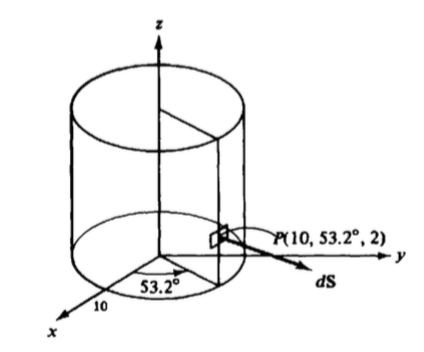
\includegraphics[width=0.99\textwidth]{./images/problems/lect02_electric_flux_area_on_cylinder.png}\\
        \end{center}
      \end{column}
      \begin{column}{0.53\textwidth}
        Determine the electric flux crossing \\
        a 1 mm $\times$ 1 mm area on the surface \\
        of the cylindrical shell at:
        \begin{equation*}
          r = 10 \; m, \;\; z = 2 \; m, \; \phi = 53.2^{o}
        \end{equation*}
     \end{column}
   \end{columns}
  \end{blockexmplque}
  \vspace{0.4cm}

\end{frame}

%
%
%

\begin{frame}{Worked example}

  At the point P:
  \begin{equation*}
     x = r  cos\phi = (10 \; m)  cos53.2^o = (10 \; m)  0.6 = 6 \; m
  \end{equation*}
  \begin{equation*}
     y = r  sin\phi = (10 \; m)  sin53.2^o = (10 \; m)  0.8 = 8 \; m
  \end{equation*}

  \vspace{0.2cm}

  The electric field $\vec{E}$ varies very little over the small given area.
  Taking it to be constant is a good approximation.\\
  Therefore, I will just substitute x = 6 m, y = 8 m, and z = 2 m
  in the given expression for $\vec{E}$:
  \begin{equation*}
   \vec{E} =
     \big\{ 2 \cdot (6\; m) \; \frac{N}{m \cdot C} \big\} \hat{x} +
     \big\{ 2 \; \frac{N}{C} - 2 \cdot (8 \; m) \frac{N}{m \cdot C} \big\} \hat{y} +
     \big\{ 4 \cdot (2\;m) \; \frac{N}{m \cdot C} \big\} \hat{z} \Rightarrow
  \end{equation*}
  \begin{equation*}
   \vec{E} =
   \big\{ 12 \hat{x} - 14 \hat{y} + 8 \hat{z} \big\} \frac{N}{C}
 \end{equation*}

\end{frame}

%
%
%

\begin{frame}{Worked example}

Now, I need to express the area $d\vec{S}$ in vector form.\\
\vspace{0.2cm}
Because the area is very small ($|d\vec{S}|$ = 1 mm$^2$) in comparison to the
size of the cylinder (r = 10 m), we can consider the area $d\vec{S}$ to be {\em planar}.\\
\vspace{0.1cm}
Also, as one can easily see, the vector $d\vec{S}$ lies on the xy plane.\\
\vspace{0.3cm}
Therefore:
\begin{equation*}
  d\vec{S} = dS_x \hat{x} + dS_y \hat{y}
\end{equation*}
where:
\begin{equation*}
   dS_x = |d\vec{S}| cos\phi = (10^{-6} \; m^2) \; cos53.2^o = 0.6 \times 10^{-6} \; m^2
\end{equation*}
\begin{equation*}
   dS_y = |d\vec{S}| sin\phi = (10^{-6} \; m^2) \; sin53.2^o = 0.8 \times 10^{-6} \; m^2
\end{equation*}
\vspace{0.2cm}
Putting everything together:
\begin{equation*}
  d\vec{S} = \big\{ 0.6 \hat{x} + 0.8 \hat{y} \big\} \times 10^{-6} \; m^2
\end{equation*}

\end{frame}

%
%
%

\begin{frame}{Worked example}

We're now ready to calculate the flux d$\Phi$ of the electric field $\vec{E}$
through the small patch $d\vec{S}$:\\
\vspace{0.2cm}
\begin{equation*}
  d\Phi = \vec{E} \cdot d\vec{S} \Rightarrow
\end{equation*}
\vspace{0.1cm}
\begin{equation*}
  d\Phi =
  \big\{ 12 \hat{x} - 14 \hat{y} + 8 \hat{z} \big\} \frac{N}{C}
   \cdot \big\{ 0.6 \hat{x} + 0.8 \hat{y} \big\} \times 10^{-6} \; m^2 \Rightarrow
\end{equation*}
\vspace{0.1cm}
\begin{equation*}
  d\Phi =
  \big\{ 12 \cdot 0.6 - 14 \cdot 0.8 + 8 \cdot 0 \big\} \times 10^{-6} \frac{N \cdot m^2}{C} =
  \big\{ 7.2 - 11.2 + 0 \big\} \times 10^{-6} \frac{N \cdot m^2}{C}
  \Rightarrow
\end{equation*}
\vspace{0.1cm}
\begin{equation*}
  d\Phi = -4 \times 10^{-6} \frac{N \cdot m^2}{C}
\end{equation*}
\vspace{0.1cm}
Q: What is the significance of the minus sign?
\end{frame}


} % Example


%
%
%

\begin{frame}{Electric flux through a closed surface}

\begin{center}
 What is the electric flux through the closed surface shown?\\
\end{center}
\vspace{0.2cm}

\begin{columns}
  \begin{column}{0.38\textwidth}
   {\small
     No charge is contained in the closed surface.\\
     \vspace{0.2cm}
     Since flux lines start from positive charges and end in negative charges,
     every line that enters the closed surface eventually exits.\\
     \vspace{0.2cm}
     Field lines that enter and field lines that exit contribute with different signs in $\oint \vec{E} d\vec{S}$
     (recall that the surface vector points outwards).\\
     \vspace{0.2cm}
     The flux is 0.
   }
   \begin{center}
   \end{center}
  \end{column}
  \begin{column}{0.62\textwidth}
    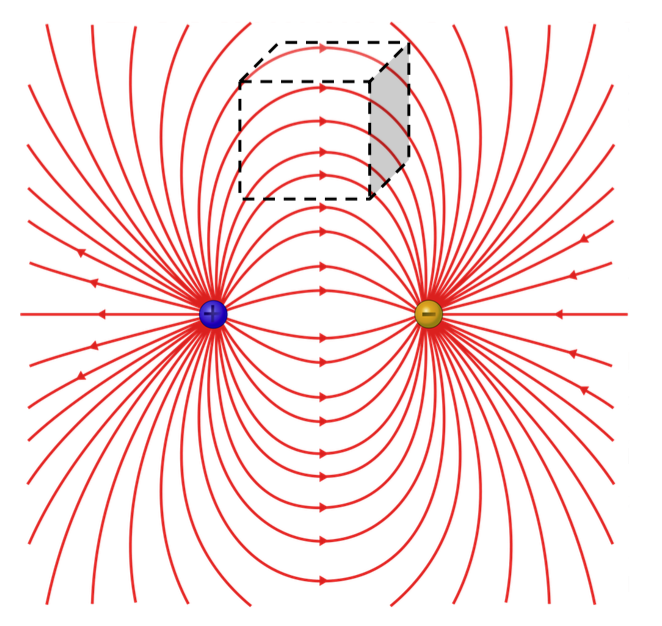
\includegraphics[width=0.90\textwidth]{./images/schematics/electric_dipole_field_lines_closed_surf_noq.png}\\
  \end{column}
\end{columns}
\end{frame}


%
%
%

\begin{frame}{Electric flux through a closed surface}

\begin{center}
 What is the electric flux through the closed surface shown?\\
\end{center}
\vspace{0.2cm}

\begin{columns}
  \begin{column}{0.38\textwidth}
   {\small
     Both a positive and an equal negative charge are contained within the closed surface.
     Certain lines originating from the positive charge can reach the negative charge without exiting the closed surface.
     Lines that do exit though the closed surface, re-enter to terminate on the negative charge. \\
     \vspace{0.2cm}
     The flux is 0 again.
   }
   \begin{center}
   \end{center}
  \end{column}
  \begin{column}{0.62\textwidth}
    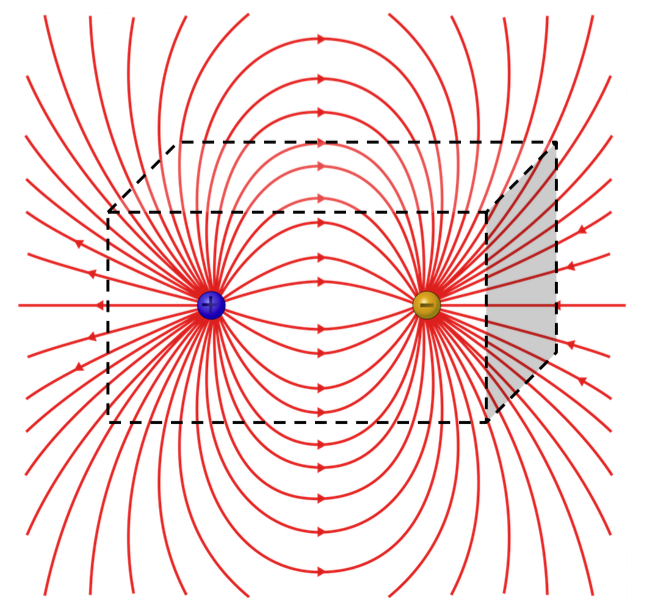
\includegraphics[width=0.90\textwidth]{./images/schematics/electric_dipole_field_lines_closed_surf_bothq.png}\\
  \end{column}
\end{columns}
\end{frame}


%
%
%

\begin{frame}{Electric flux through a closed surface}

\begin{center}
 What is the electric flux through the closed surface shown?\\
\end{center}
\vspace{0.2cm}

\begin{columns}
  \begin{column}{0.38\textwidth}
   {\small
     All field lines are exiting.
     The flux is non-zero and positive.
   }
   \begin{center}
   \end{center}
  \end{column}
  \begin{column}{0.62\textwidth}
    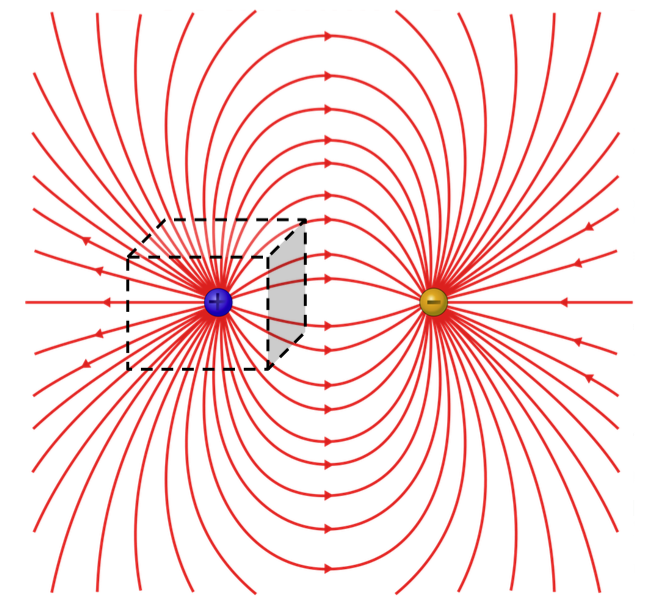
\includegraphics[width=0.90\textwidth]{./images/schematics/electric_dipole_field_lines_closed_surf_posq.png}
  \end{column}
\end{columns}
\end{frame}


%
%
%

\begin{frame}{Electric flux through a closed surface}

\begin{center}
 What is the electric flux through the closed surface shown?\\
\end{center}
\vspace{0.2cm}

\begin{columns}
  \begin{column}{0.38\textwidth}
   {\small
     Now all field lines are entering.
     The flux is non-zero. It has the same value as in the previous page, but now it is negative.
   }
   \begin{center}
   \end{center}
  \end{column}
  \begin{column}{0.62\textwidth}
    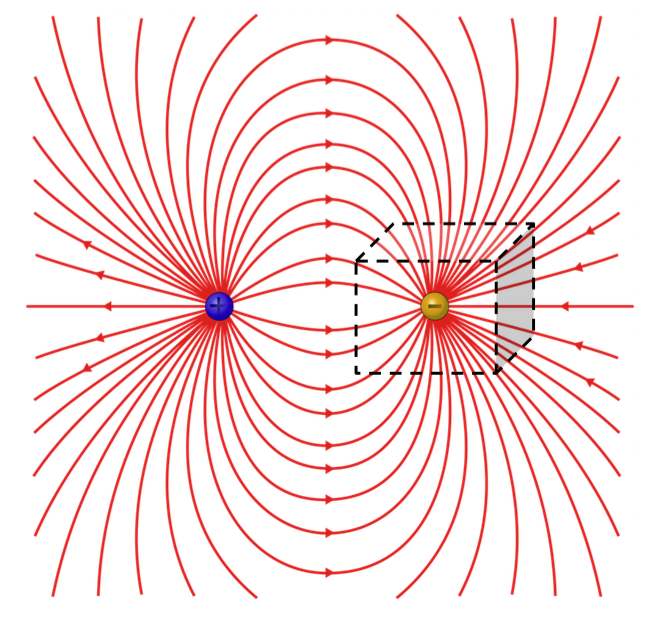
\includegraphics[width=0.90\textwidth]{./images/schematics/electric_dipole_field_lines_closed_surf_negq.png}\\
  \end{column}
\end{columns}
\end{frame}


%
%
%

\begin{frame}{Gauss' law}

In the previous few slides, the {\em essence} of {\bf Gauss' law} was illustrated.\\
\vspace{0.3cm}

\begin{columns}
  \begin{column}{0.33\textwidth}
   \begin{center}
    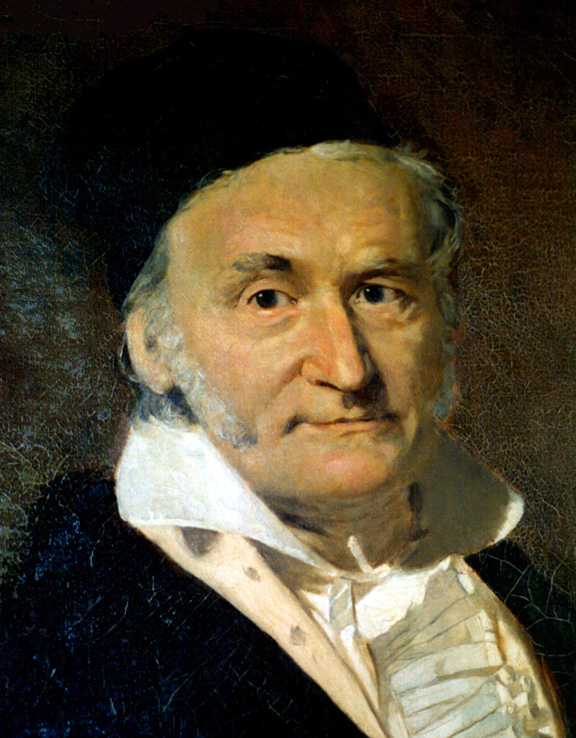
\includegraphics[width=0.90\textwidth]{./images/people/gauss.jpg}\\
    \vspace{0.2cm}
    {\scriptsize
      Carl Friedrich Gauss\\ (1777-1855)\\ German mathematician\\
    }
   \end{center}
  \end{column}
  \begin{column}{0.67\textwidth}
      {\em \bf
       The electric flux $\Phi_{E} = \oint \vec{E} d\vec{S}$ through a closed surface
       is related to the net charge $Q_{enc}$ enclosed within the surface.\\
      }
      \vspace{0.4cm}
      As it turns out, this relation is simply:
      \begin{equation*}
         {\color{red}
          \Phi_{E} = \frac{Q_{enc}}{\epsilon_0}
         }
      \end{equation*}

      It doesn't matter how elaborate the shape of the surface or the enclosed
      charge distribution (and the resulting field) may be:\\
      The above simple relation {\bf always holds}!\\
  \end{column}
\end{columns}
\end{frame}


%
% Worked example
%

{
\problemslide

%
%
%

\begin{frame}{Worked example}

  \begin{blockexmplque}{Question}
    \begin{columns}
      \begin{column}{0.40\textwidth}
        \begin{center}
          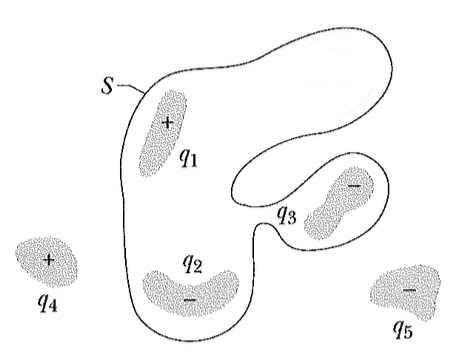
\includegraphics[width=0.99\textwidth]{./images/problems/lect02_enclosed_charges.png}\\
        \end{center}
      \end{column}
      \begin{column}{0.60\textwidth}
        The figure on the left shows 5 charged lumps of a material.
        The cross-section of the surface S is indicated.\\
        What is the {\em net electric flux} through the surface if:\\
        \begin{itemize}
         \item q$_1$ = q$_4$ = 3.1 nC,
         \item q$_2$ = q$_5$ = -5.9 nC, and
         \item q$_3$ = -3.1 nC?
        \end{itemize}
     \end{column}
   \end{columns}
  \end{blockexmplque}
  \vspace{0.2cm}
  \begin{equation*}
  \Phi =
    \frac{Q_{enc}}{\epsilon_0} =
    \frac{q_1+q_2+q_3}{\epsilon_0} =
    \frac{(3.1 - 5.9 - 3.1) \times 10^{-9} \; C}{8.85 \times 10^{-12} \; C^2/(N \cdot m^2)} =
    -0.67 \times 10^{3} \frac{N \cdot m^2}{C}
  \end{equation*}

\end{frame}

} % Example

%
%
%

\begin{frame}{Gauss' law - Derivation for a simple case}

%\begin{center}
We will derive Gauss' law for a very simple case: A single charge Q in the centre of a sphere of radius R.
%\end{center}

\begin{columns}
  \begin{column}{0.34\textwidth}
   \begin{center}
    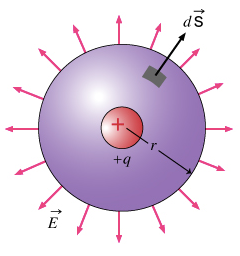
\includegraphics[width=0.85\textwidth]{./images/schematics/gauss_law_S.png}
    \begin{equation*}
        \vec{E}(\vec{r}) = \frac{Q}{4\pi\epsilon_0 r^{2}} \hat{r}
    \end{equation*}
    \begin{equation*}
        d\vec{S} = dS \hat{r}
    \end{equation*}
   \end{center}
  \end{column}
  \begin{column}{0.66\textwidth}
    \begin{equation*}
        \Phi_E = \oint_{sphere} \vec{E} \cdot d\vec{S} \Rightarrow
    \end{equation*}
    \begin{equation*}
        \Phi_E = \oint_{sphere} \big( \frac{Q}{4\pi\epsilon_0 R^{2}} \hat{r} \big) \cdot \big( dS \hat{r} \big) \xRightarrow {\hat{r}\cdot\hat{r}=1}
    \end{equation*}
    \begin{equation*}
        \Phi_E = \frac{Q}{4\pi\epsilon_0 R^{2}} \oint_{sphere} dS \Rightarrow
    \end{equation*}
    \begin{equation*}
        \Phi_E = \frac{Q}{4\pi\epsilon_0 R^{2}} 4\pi R^{2} \Rightarrow
    \end{equation*}
    \begin{equation*}
    {\bf \color{magenta}
        \Phi_E = \frac{Q}{\epsilon_0}
    }
    \end{equation*}
  \end{column}
\end{columns}
\end{frame}


%
%
%

\begin{frame}{Gauss' law - Generalisation for any surface}

Although the law was derived for a very simple case, it is a {\bf general result}.\\
\vspace{0.2cm}

\begin{columns}
  \begin{column}{0.34\textwidth}
   \begin{center}
    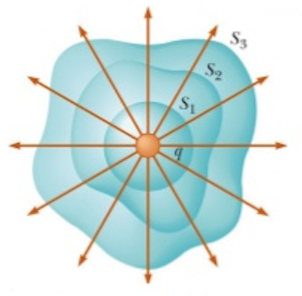
\includegraphics[width=0.98\textwidth]{./images/schematics/gauss_law_generalisation_geom_0.png}\\
   \end{center}
  \end{column}
  \begin{column}{0.66\textwidth}
    The same result would have been obtained
    \begin{itemize}
     \item if the charge was not in the centre but in any other position within the sphere, or
     \item if I had any other closed surface shape instead of a sphere.
    \end{itemize}
  \end{column}
\end{columns}

Only one thing matters for the calculation of $\Phi_E$: The {\bf net charge within the surface}.

\end{frame}


%
%
%

\begin{frame}{Gauss' law - Generalisation for any surface}

\begin{columns}
  \begin{column}{0.34\textwidth}
   \begin{center}
    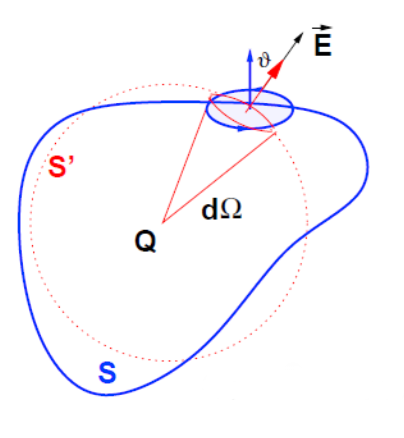
\includegraphics[width=0.90\textwidth]{./images/schematics/gauss_law_generalisation_geom_1.png}\\
    {\scriptsize
     Consider element $dS$ on a general surface $S$ and the corresponding element $dS^{\prime}$ on a sphere $S^{\prime}$,
     both covering the same solid angle $d\Omega$
    }
   \end{center}
  \end{column}
  \begin{column}{0.66\textwidth}
     By definition, on the spherical surface $S^{\prime}$:
     \begin{equation*}
       d\Omega = \frac{dS^{\prime}}{r^{2}} \Rightarrow dS^{\prime} = r^{2} d\Omega
     \end{equation*}
     By construction:
     \begin{equation*}
       dS^{\prime} = dS cos\theta \Rightarrow dS = \frac{dS^{\prime}}{cos\theta} \Rightarrow dS = \frac{r^{2} d\Omega}{cos\theta}
     \end{equation*}
     So, the flux $\Phi_E$ through the general surface $S$ is
     \begin{equation*}
       \Phi_E = \int_{S} \vec{E} \cdot d\vec{S} = \int_{S} E dS cos\theta
          = \int_{\Omega} E \frac{r^{2} d\Omega}{\cancel{cos\theta}} \cancel{cos\theta} =
     \end{equation*}
     \begin{equation*}
        \int_{\Omega} E r^{2} d\Omega = \int_{S^{\prime}} E dS^{\prime}
        = \int_{S^{\prime}} \vec{E} d\pvec{S}' = \Phi_E^{sphere} = \frac{Q}{\epsilon_0}
     \end{equation*}
  \end{column}
\end{columns}
\end{frame}


%
%
%

\begin{frame}{Gauss' law - Generalization for any charge distribution}


Our result for a {\em single charge} enclosed by an arbitrary closed surface S is:
\begin{equation*}
   \oint_{S} \vec{E} \cdot d\vec{S} = \frac{Q}{\epsilon_0}
\end{equation*}

What is the {\bf form of Gauss' law if the surface S encloses an array of charges} (or a continuous charge distribution)?
The result can be obtained via a straightforward application of the superposition principle.\\

\begin{equation*}
  \left.
     \begin{array}{l}
      \oint_{S} \vec{E_{1}} \cdot d\vec{S} = \frac{Q_{1}}{\epsilon_0}\\
      \\
      \oint_{S} \vec{E_{2}} \cdot d\vec{S} = \frac{Q_{2}}{\epsilon_0}\\
      \\
      ...                                                      \\
      \\
      \oint_{S} \vec{E_{n}} \cdot d\vec{S} = \frac{Q_{n}}{\epsilon_0}
     \end{array}
  \right\}
%  \oint_{S} (\vec{E_{1}}+\vec{E_{2}}+...+\vec{E_{n}}) d\vec{S} = \frac{Q_{1}+Q_{2}+...+Q_{n}}{\epsilon_0} \Rightarrow
  \oint_{S} (\sum_{i=1}^{n}\vec{E_{i}}) \cdot d\vec{S} = \frac{\sum_{i=1}^{n}Q_{i}}{\epsilon_0} \Rightarrow
  \oint_{S} \vec{E} \cdot d\vec{S} = \frac{Q_{enc}}{\epsilon_0}
\end{equation*}

\end{frame}


%
%
%

\begin{frame}{Integral form of Gauss' law}

Our result for any array of charges (or continuous charge distribution), with net charge $Q_{enc}$,
enclosed by an arbitrary closed surface S is:
\begin{equation*}
  \oint \vec{E} \cdot d\vec{S} = \frac{Q_{enc}}{\epsilon_0}
\end{equation*}

This is known as the {\bf \underline{integral form} of Gauss' law}.\\
\vspace{0.2cm}

This form is useful in cases where the problem at hand has a symmetry.\\
The symmetry can be exploited to simplify the calculation of the integral.\\

\end{frame}



%
% Worked example
%

{
\problemslide

%
% Another
%

\begin{frame}{Worked example (Planar symmetry)}

  \begin{blockexmplque}{Question}
    The figure on the left shows two large, parallel, non-conducting sheets,
    each with a fixed uniform charge on one side.\\
    \begin{columns}
      \begin{column}{0.20\textwidth}
        \begin{center}
          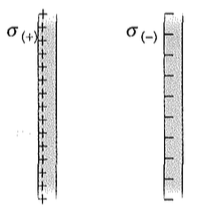
\includegraphics[width=0.99\textwidth]{./images/problems/lect02_2_charged_planes.png}\\
        \end{center}
      \end{column}
      \begin{column}{0.80\textwidth}
        The magnitudes of the surface charge densities are\\
        $\sigma_{(+)}$ = 6.8 $\mu$C/m$^2$ for the positively charged sheet, and
        $\sigma_{(-)}$ = - 4.3 $\mu$C/m$^2$ for the negatively charged sheet.\\
        Find the electric field $\vec{E}$
        (a) to the left of the sheets,
        (b) between the sheets, and
        (c) to the right of the sheets.
     \end{column}
   \end{columns}
  \end{blockexmplque}
  \vspace{0.4cm}

  Note: We will revisit this example when we study the {\bf parallel plate capacitor}
  in Lecture 4.\\

\end{frame}

%
%
%

\begin{frame}{Worked example (Planar symmetry)}

  Consider an infinite positively charged plane with surface charge density
  $\sigma$ and the (appropriately chosen)
  cylindrical {\em Gaussian} surface shown below.\\

  \begin{columns}
   \begin{column}{0.60\textwidth}
    The symmetry of the problem indicates that $\vec{E}$ is
    {\bf perpendicular to the sheet}: There is no
    flux through the curved surface but only through the 2 circular end caps.\\
    \vspace{0.2cm}
    Additionally, because the plane is positively charged, the field $\vec{E}$
    is directed outwards.\\
   \end{column}
   \begin{column}{0.40\textwidth}
    \begin{center}
      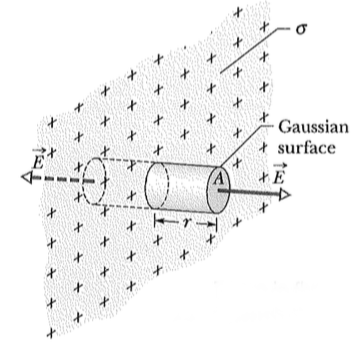
\includegraphics[width=0.70\textwidth]{./images/problems/lect02_charged_plane_3d.png}\\
    \end{center}
   \end{column}
  \end{columns}
  The surface charge enclosed by the Gaussian surface is $Q_{enc} = \sigma A$.\\
  \vspace{0.2cm}
  Therefore, applying Gauss' law, we get:
  \begin{equation*}
    \oint \vec{E} \cdot d\vec{S} = \frac{Q_{enc}}{\epsilon_0} \Rightarrow
    EA + EA = \frac{\sigma A}{\epsilon_0} \Rightarrow
    {\color{red}
      E = \frac{\sigma}{2\epsilon_0}
    }
  \end{equation*}
  The electric field stays the same for any point, irrespectively of its distance from the plane.

\end{frame}

%
%
%

\begin{frame}{Worked example (Planar symmetry)}

Repeating the exercise for a negatively charged plane yield of the same magnitude.
with the difference that it would point inwards.\\
\vspace{0.2cm}

For the case of the 2 parallel plates, the electric field $\vec{E}$ anywhere in
space is given by the superposition of 2 fields:\\
\vspace{0.2cm}
\begin{itemize}
  \item The field $\vec{E}_{(+)}$, due to the positively charged plane, with direction
        away from that plane and magnitude:
        \begin{equation*}
            E_{(+)} =
              \frac{\sigma_{(+)}}{2\epsilon_0} =
              \frac{6.8 \times 10^{-6} \; C/m^2}{2(8.85 \times 10^{-12} \; C/(N \cdot m^2))} =
              3.84 \times 10^{5} N/C
        \end{equation*}
  \item The field $\vec{E}_{(-)}$, due to the positively charged plane, with direction
        away from that plane and magnitude:
        \begin{equation*}
            E_{(-)} =
              \frac{\sigma_{(-)}}{2\epsilon_0} =
              \frac{4.3 \times 10^{-6} \; C/m^2}{2(8.85 \times 10^{-12} \; C/(N \cdot m^2))} =
              2.43 \times 10^{5} N/C
        \end{equation*}
\end{itemize}

\end{frame}

%
%
%

\begin{frame}{Worked example (Planar symmetry)}

  \begin{columns}
   \begin{column}{0.50\textwidth}
     We can now work out the electric field on the left of the planes,
     between the planes, and on the right of the planes.
   \end{column}
   \begin{column}{0.50\textwidth}
    \begin{center}
      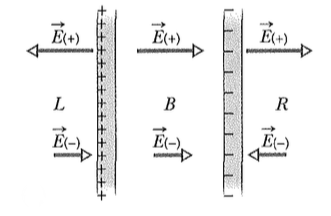
\includegraphics[width=0.90\textwidth]{./images/problems/lect02_2_charged_planes_solution.png}\\
    \end{center}
   \end{column}
  \end{columns}

     \begin{itemize}
        \item
          On the {\bf left} of the planes:\\
          $E_{L} = E_{(+)} - E_{(-)} = 1.4 \times 10^{5} \; N/C$
          directed to the left.\\
          \vspace{0.2cm}
        \item
          {\bf Between} the planes:\\
          $E_{B} = E_{(+)} + E_{(-)} = 6.3 \times 10^{5} \; N/C$
          directed to the right.\\
          \vspace{0.2cm}
        \item
          On the {\bf right} of the planes:\\
          $E_{R} = E_{(+)} - E_{(-)} = 1.4 \times 10^{5} \; N/C$
          directed to the right.\\
      \end{itemize}

\end{frame}


%
% Another
%

\begin{frame}{Worked example (Cylindrical symmetry)}

\begin{blockexmplque}{Question}
A long, straight, thin plastic rod is uniformly charged with +10 nC/m.
Calculate the magnitude of the electric field at 10 cm away from the rod.
What is the direction of the electric field at any point away from the rod?
\end{blockexmplque}
\vspace{0.4cm}

Consider a cylindrical surface with the rod running along its axis.\\
\vspace{0.2cm}

Gauss' law in integral form is:
\begin{equation*}
 \oint \vec{E}(r) \cdot d\vec{S} = \frac{Q_{encl}}{\epsilon_0}
\end{equation*}

Assuming the rod is infinitely long (i.e. ignoring fringe effects)
the electric field is everywhere perpendicular to the rod and points away from it.
Therefore, all the flux is going out of the sides of the cylinder.\\

\end{frame}

%
%
%

\begin{frame}{Worked example (Cylindrical symmetry)}

For a length L and linear charge density $\lambda$:

\begin{columns}
  \begin{column}{0.45\textwidth}
   \begin{center}
     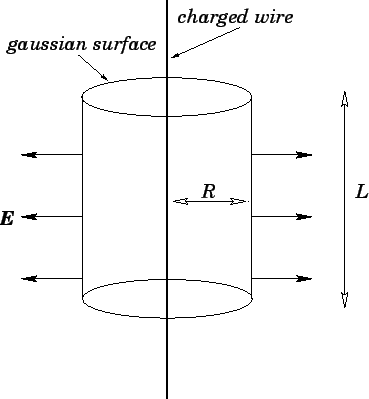
\includegraphics[width=0.65\textwidth]{./images/problems/lect1_charged_rod.png}\\
   \end{center}
  \end{column}
  \begin{column}{0.55\textwidth}

    \begin{equation*}
      \oint \Big( E(r) \hat{r} \Big) \cdot \Big( dS \hat{r} \Big) = \frac{\lambda L}{\epsilon_0} \Rightarrow
    \end{equation*}

    \begin{equation*}
      E(r) 2\pi r L = \frac{\lambda L}{\epsilon_0} \Rightarrow
    \end{equation*}

    \begin{equation*}
      E(r) = \frac{\lambda}{2 \pi \epsilon_0 r}
    \end{equation*}

  \end{column}
\end{columns}

\vspace{0.3cm}

At the given distance away from the rod (10 cm), the magnitude of the electric field is:

\begin{equation*}
 E = 2 \cdot (9.0 \times 10^9 \; \frac{N \cdot m^2}{C^2}) \frac{10 \times 10^{-9} \; C/m}{0.1 \; m} \Rightarrow
 E = 1.8 \; kV/m
\end{equation*}

\end{frame}


%
% Another
%

\begin{frame}{Worked example (Spherical symmetry)}

  \begin{blockexmplque}{Question}
    A solid non-conductive sphere with radius R is uniformly charged and carries total charge Q.
    Calculate the electric field E at radius r from its centre for the following two cases:
    \begin{enumerate}
       \item Inside the sphere (r $<$ R).
       \item On the surface or outside the sphere (r $\geq$ R).
    \end{enumerate}
    How is the result for case 2 above related to that for a point charge Q at
    the origin? \\
  \end{blockexmplque}
  \vspace{0.4cm}

  The charge density is:
  \begin{equation*}
    \rho = \frac{Q}{\tau} = \frac{Q}{4\pi R^3 /3} = \frac{3Q}{4\pi R^3}
  \end{equation*}

\end{frame}

%
%
%

\begin{frame}{Worked example (Spherical symmetry)}

  Exploiting the spherical symmetry of the problem,
  the flux of the electric field at any distance r is:
  \begin{equation*}
    \Phi(r) = 4\pi r^2 E(r)
  \end{equation*}

  From Gauss' law:
  \begin{equation*}
    \Phi(r) = \frac{Q_{encl}(r)}{\epsilon_0}
  \end{equation*}

  Therefore:
  \begin{equation*}
    4\pi r^2 E(r) = \frac{Q_{encl}(r)}{\epsilon_0}
  \end{equation*}
  \begin{equation*}
    E(r) = \frac{Q_{encl}(r)}{4 \pi \epsilon_0 r^2}
  \end{equation*}

\end{frame}

%
%
%

\begin{frame}{Worked example (Spherical symmetry)}

  {\bf For $r < R$:}

  \begin{equation*}
    Q_{encl}(r) =  \rho \tau(r) = \frac{3Q}{4\pi R^3} \cdot \frac{4\pi r^3}{3} = Q \frac{r^3}{R^3}
  \end{equation*}

  \begin{equation*}
    E(r) = \frac{Q \frac{r^3}{R^3}}{4 \pi \epsilon_0 r^2} = \frac{Q}{4 \pi \epsilon_0 R^3} r
  \end{equation*}

  {\bf For $r \ge R$:}

  \begin{equation*}
    Q_{encl}(r) =  Q
  \end{equation*}

  \begin{equation*}
    E(r) = \frac{Q}{4 \pi \epsilon_0 r^2}
  \end{equation*}

  The result for the case of $r \ge R$  is identical to that for point charge Q at the origin.

\end{frame}

} % Example

%
%
%

\begin{frame}{Integral and differential forms of Gauss' law}

Our result for any array of charges (or continuous charge distribution), with net charge $Q_{enc}$,
enclosed by an arbitrary closed surface S is:
\begin{equation*}
  \oint \vec{E} \cdot d\vec{S} = \frac{Q_{enc}}{\epsilon_0}
\end{equation*}

This is known as the {\bf \underline{integral form} of Gauss' law}.\\
\vspace{0.2cm}

This form is useful in cases where the problem at hand has a symmetry.\\
The symmetry can be exploited to simplify the calculation of the integral.\\
Will will see several examples of the above in the workshops.\\
\vspace{0.2cm}

It is very useful to obtain Gauss' law in its {\bf \underline{differential form}}.\\
This is a more practical form for the analytical or numerical solution of problems
that do not have a symmetry that we can exploit.\\
\vspace{0.2cm}

Before we can proceed, we need to continue brushing up our calculus skills.

\end{frame}



% starting reminder
{
\reminderslide

%
%
%

\begin{frame}{Reminder: Gradient, Divergence, Curl and all that}

\begin{itemize}
  \item The $\vec\nabla$ ({\em nabla}) operator
    \begin{equation*}
       \vec{\nabla} = (\frac{\partial}{\partial x}, \frac{\partial}{\partial y}, \frac{\partial}{\partial z})
    \end{equation*}
  \item The nabla operator is a kind of a vector
    \begin{itemize}
        \item It is a {\em vector operator} that acts upon the quantity on the right
        \item It appears as a vector as long as we do not make a distinction between "acting upon" and "multiplying"
    \end{itemize}
  \vspace{0.3cm}
  \item Just as we have 3 kinds of vector multiplications (with scalar, dot product, cross product),
        we have 3 ways the nabla operator can act
    \begin{itemize}
       \item $\vec\nabla$ (a scalar function) $\rightarrow$ {\bf gradient}
       \item $\vec\nabla$ $\cdot$ (a vector function) $\rightarrow$ {\bf divergence}
       \item $\vec\nabla$ $\times$ (a vector function) $\rightarrow$ {\bf curl}
    \end{itemize}
\end{itemize}

\end{frame}


%
%
%

\begin{frame}{Reminder: Gradient, Divergence, Curl and all that}

\underline{\bf Gradient}:
This is a {\bf generalization to many dimensions} of the concept of the derivative of a 1-dimensional function.\\
\vspace{0.1cm}
Let $f(x,y)$ be a scalar field in a 2-dimensional space. Its gradient is:
\begin{equation*}
   \vec\nabla f(x,y) =
     \Big(
       \frac{\partial f(x,y)}{\partial x},
       \frac{\partial f(x,y)}{\partial y}
     \Big)
\end{equation*}

\begin{columns}
  \begin{column}{0.50\textwidth}
    Like the usual derivative, $\vec\nabla f(x,y)$ tells us how fast $f(x,y)$ changes as we move in space.\\
    \vspace{0.1cm}
    Notice that $\vec\nabla f(x,y)$ is a vector.
    It tells us, not only how fast $f(x,y)$ changes, but also the {\bf direction of the steepest ascent}.\\
    \vspace{0.1cm}
    Similarly for 3 or more dimensions.
  \end{column}
  \begin{column}{0.50\textwidth}
   \begin{center}
     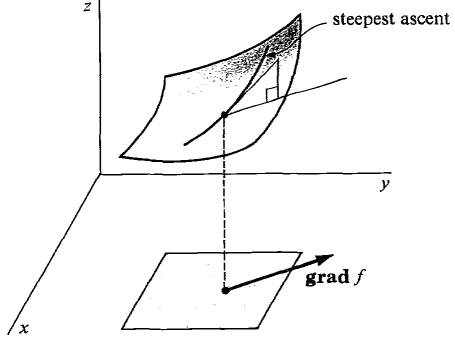
\includegraphics[width=0.85\textwidth]{./images/schematics/gradient_steepest_ascent.png}\\
   \end{center}
  \end{column}
\end{columns}

\end{frame}

%
%
%

\begin{frame}{Reminder: Gradient, Divergence, Curl and all that}

In the previous slide, we used a {\bf partial derivative}.
It is worth stopping to make sure you all understand what this is.
\vspace{0.1cm}

Consider a function f of several variables x,y,z,... Notice that\\
\begin{center}
{\color{red}
 {\Large
  $\frac{\partial f(x,y,z,...)}{\partial x}$
 }
 {\bf is not the same as}
 {\Large
  $\frac{df(x,y,z,...)}{dx}$\\
 }
}
\end{center}

\vspace{0.2cm}
A partial derivative, with respect to x, of a function of several variables, e.g. f(x,y,z,...),
is the derivative with respect to x {\bf while all other variables are held constant}.\\

\vspace{0.2cm}
On the other hand, the total derivative takes into account, not only the change of the function as x changes,
but also {\bf adds in all the changes due to the indirect dependencies}:
\begin{equation*}
   \frac{df(x,y,z,...)}{dx} =
     \frac{\partial f(x,y,z,...)}{\partial x} +
     \frac{\partial f(x,y,z,...)}{\partial y} \cdot \frac{\partial y}{\partial x} +
     \frac{\partial f(x,y,z,...)}{\partial z} \cdot \frac{\partial z}{\partial x} + ...
\end{equation*}

\end{frame}


%
%
%

\begin{frame}{Reminder: Gradient, Divergence, Curl and all that}

\underline{\bf Divergence}:
Let $\vec{F}(x,y)=\Big(F_{x}(x,y), \; F_{y}(x,y) \Big)$
be a vector field in a 2-dimensional space. Its divergence is given by:
\begin{equation*}
   \vec\nabla \cdot \vec{F}(x,y) =
       \frac{\partial F_{x}(x,y)}{\partial x} +
       \frac{\partial F_{y}(x,y)}{\partial y}
\end{equation*}
Similarly for 3 or more dimensions.\\
\vspace{0.1cm}

\begin{columns}
  \begin{column}{0.40\textwidth}
    Notice that the divergence of a vector field is a scalar.\\
    Its value for a particular point expresses the magnitude of the vector field's source (or sink) at that point.
  \end{column}
  \begin{column}{0.60\textwidth}
   \begin{center}
     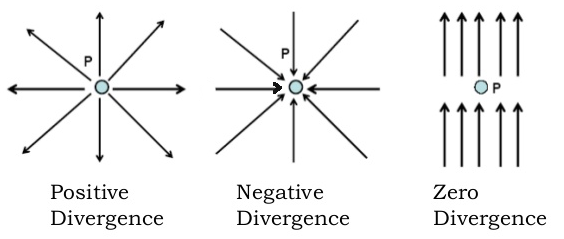
\includegraphics[width=0.98\textwidth]{./images/schematics/divergence_examples.png}\\
   \end{center}
  \end{column}
\end{columns}

\vspace{0.2cm}
\underline{\bf Curl}: This won't be introduced till later so let's forget it for now.

\end{frame}


%
%
%

\begin{frame}{Reminder: Gradient, Divergence, Curl and all that}

\begin{columns}
  \begin{column}{0.25\textwidth}
   \begin{center}
     {\bf Confused?}\\
     \vspace{0.3cm}
     {\small
      Here is a piece of advice that comes from Feynman.\\
     }
     \vspace{0.3cm}
     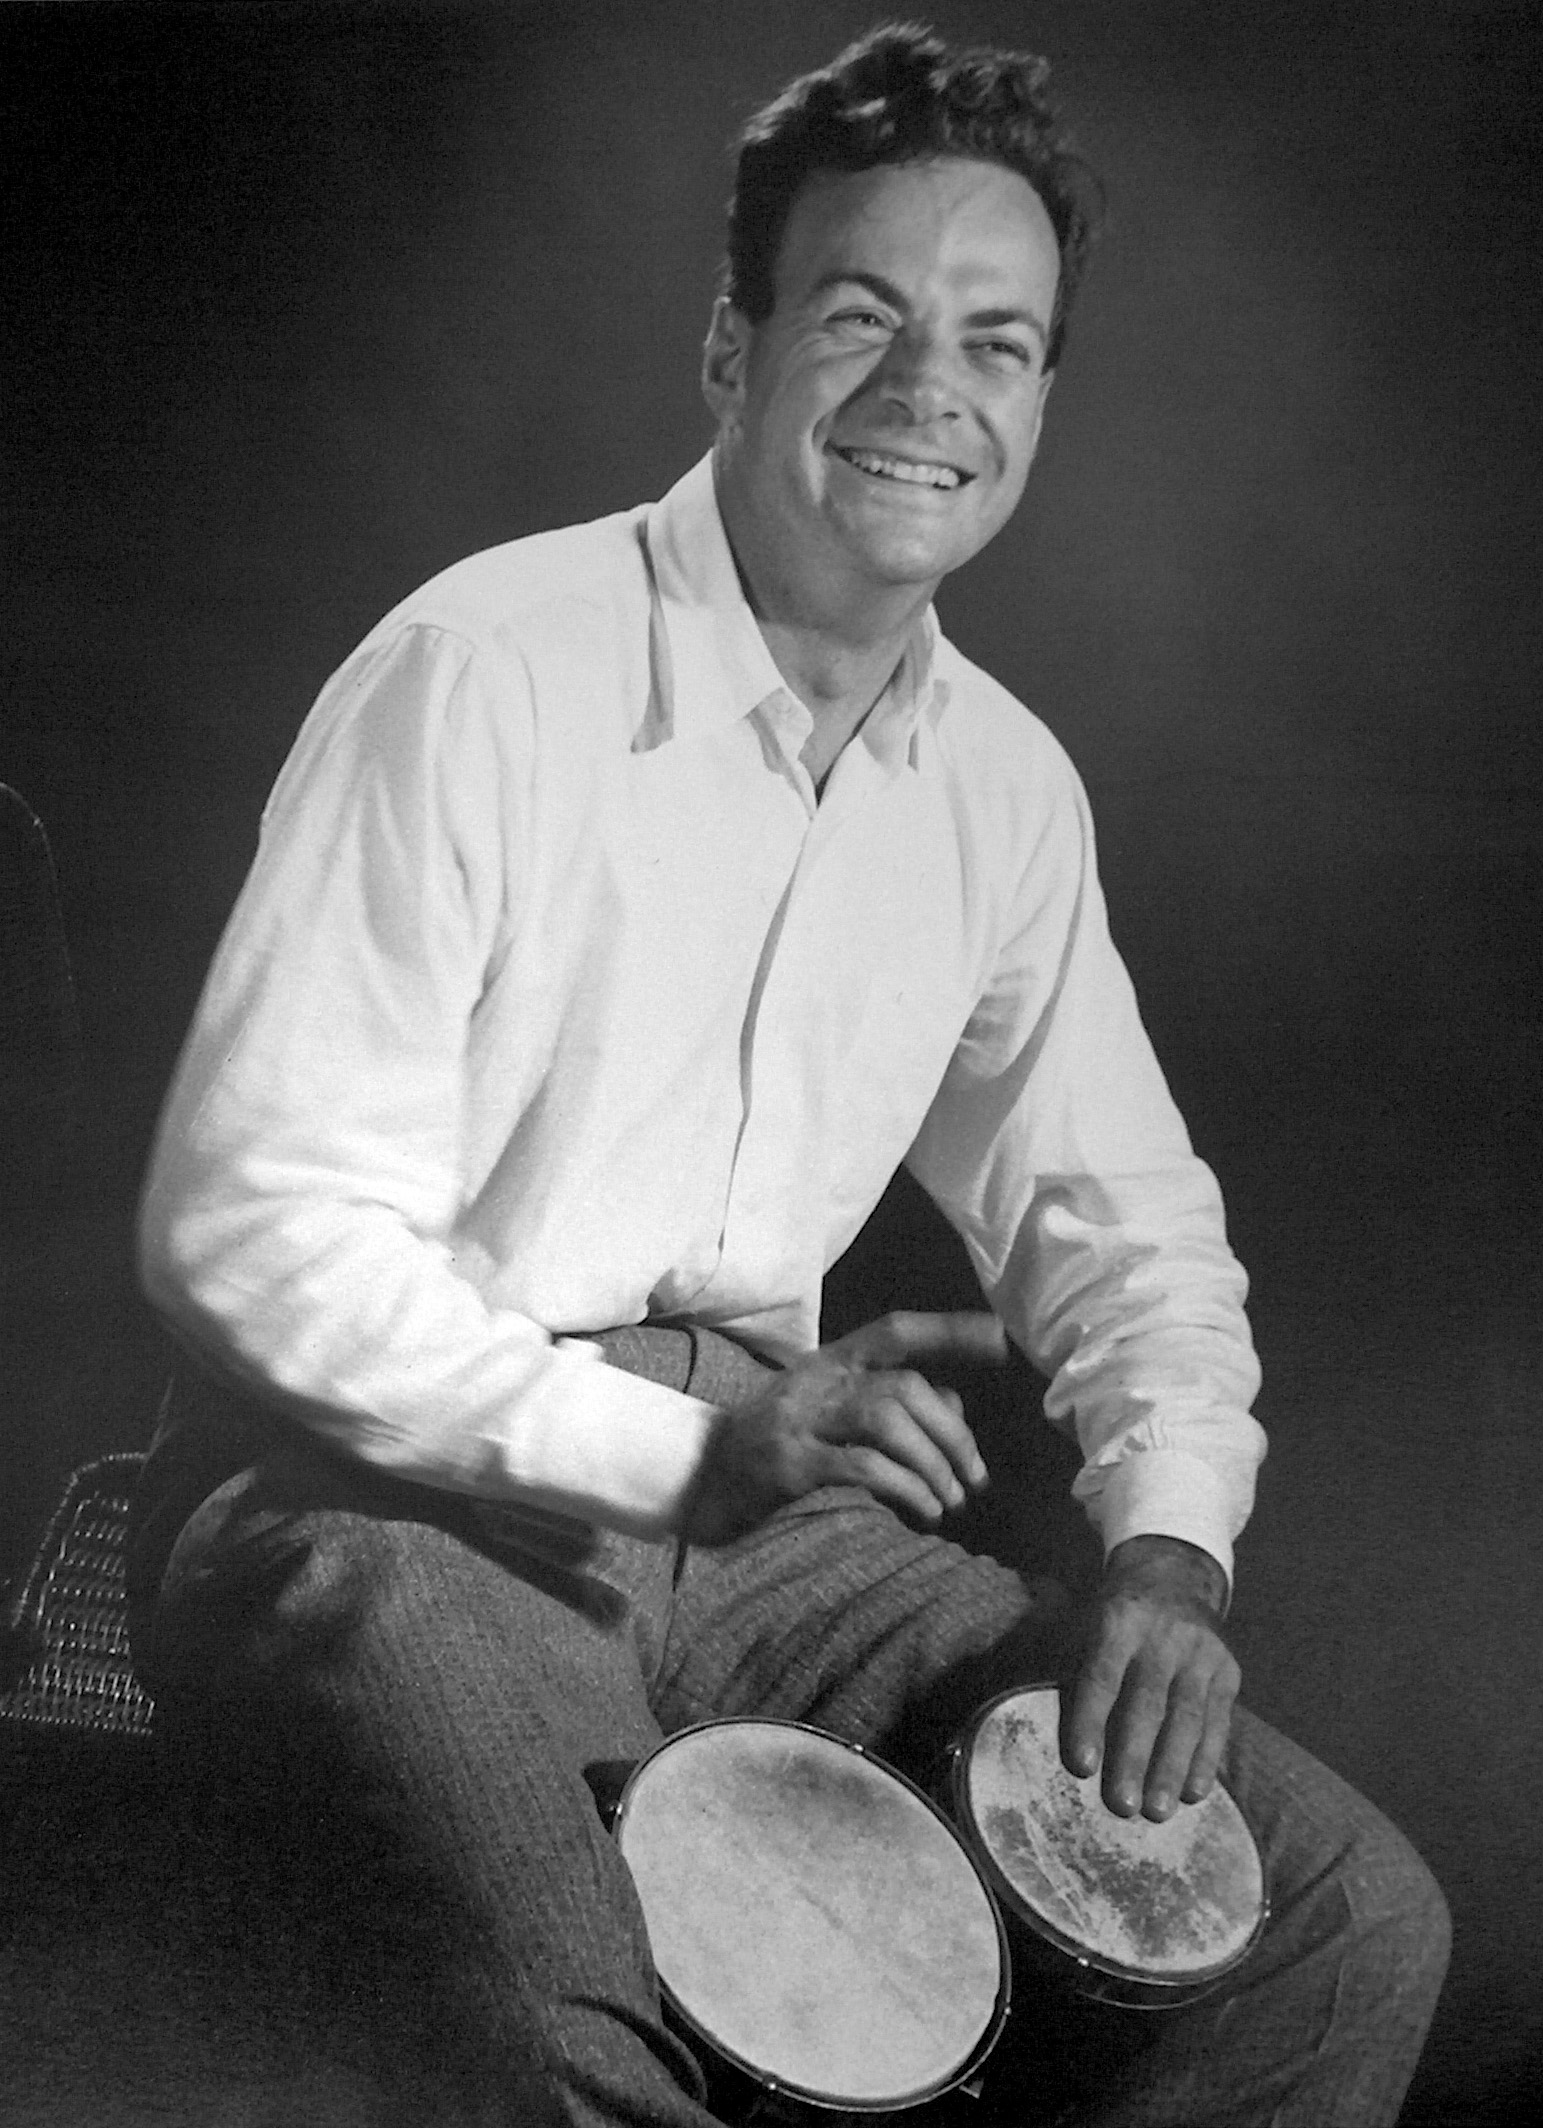
\includegraphics[width=0.99\textwidth]{./images/people/feynman_bongos2.jpg}\\
   \end{center}
  \end{column}
  \begin{column}{0.75\textwidth}
    \begin{itemize}
    {\scriptsize
      \item If you are solving a particular problem where $\vec{\nabla} \vec{E}$ appears,
            {\bf do not just stare at it} if you are not quite sure what it means or if it confuses you.
      \item This is a nice compact notation that is supposed to make our lives easier,
            not more difficult.
      \item But it takes a while to get used to compact notations and be sure that we truly understand what they mean
      \item If you find that $\vec{\nabla} \vec{E}$ confuses you, write it out as
        \begin{equation*}
         \vec{\nabla} \cdot \vec{E} = \frac{\partial E_{x}}{\partial x} + \frac{\partial E_{y}}{\partial y} + \frac{\partial E_{z}}{\partial z}
        \end{equation*}
      \item There is {\bf no shame at writing the components and not using the fancy compact notation}
    }
    \end{itemize}

    \begin{center}
    {\scriptsize
     Marking your scripts, I may excuse you for being confused by $\vec{\nabla} \cdot \vec{E}$.\\
     But not for ignoring Feynman's advice!
    }
    \end{center}

  \end{column}
\end{columns}

\end{frame}


%
%
%

\begin{frame}{Reminder: Gauss' theorem (Divergence theorem)}

\begin{center}
  Gauss' theorem: {\bf Not to be confused with Gauss' law} we saw earlier.
\end{center}

\begin{columns}
  \begin{column}{0.35\textwidth}
   \begin{center}
     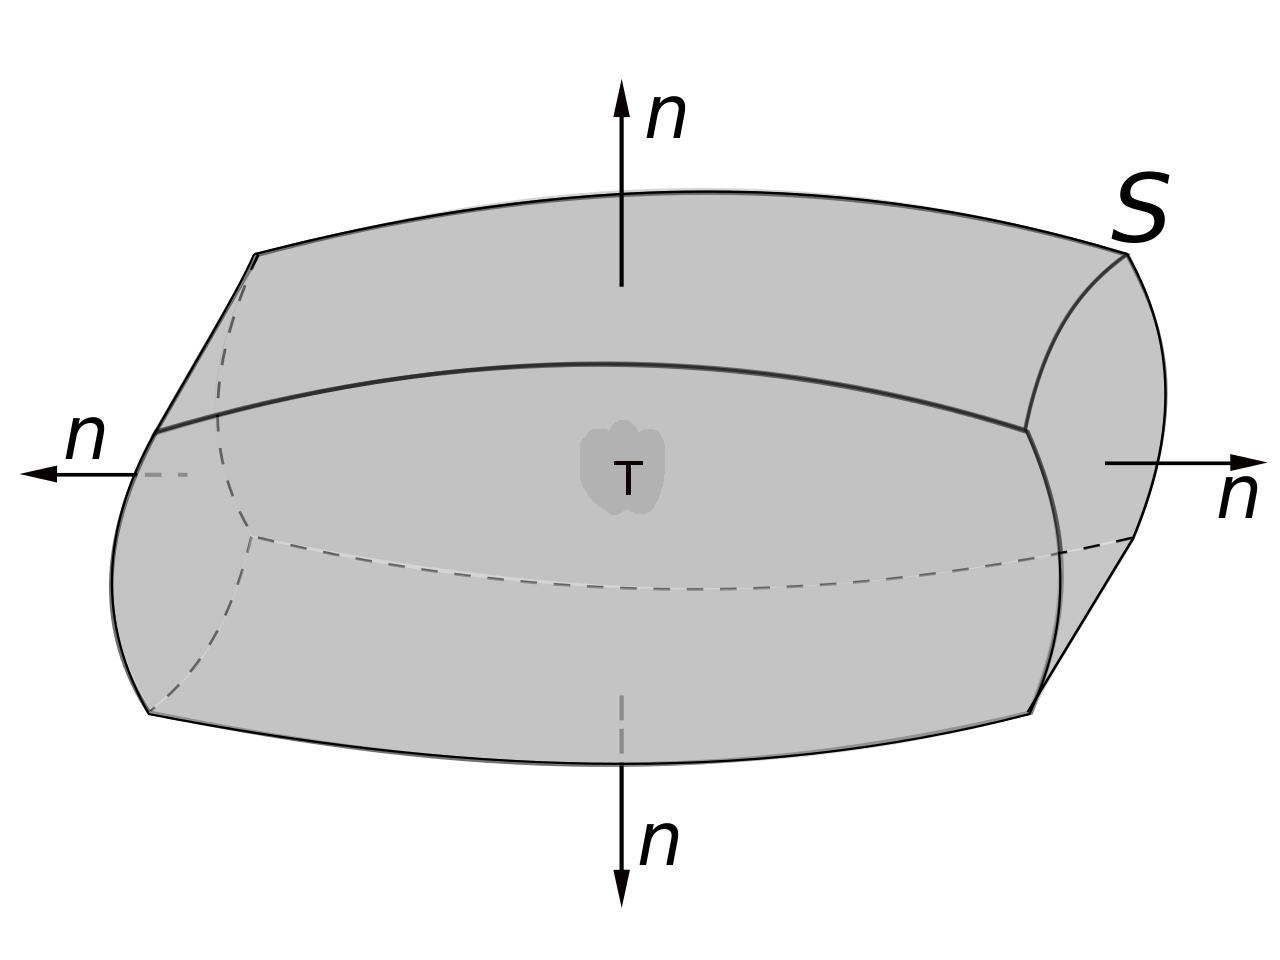
\includegraphics[width=0.95\textwidth]{./images/schematics/divergence_theorem_tau.png}\\
   \end{center}
  \end{column}
  \begin{column}{0.65\textwidth}
     \begin{itemize}
       \item Assume a volume $\tau$ whose boundary is the closed surface S
       \item Assume a vector field $\vec{F}$ which is
        \begin{itemize}
           \item defined anywhere in $\tau$
           \item continuous / differentiable anywhere in $\tau$
        \end{itemize}
     \end{itemize}
  \end{column}
\end{columns}

%\begin{block}{}
 The integral of the flux of the field $\vec{F}$ over the closed surface S is
 equal to the integral of the divergence of $\vec{F}$ in the volume $\tau$\\
 \begin{equation*}
   \oint_{S} \vec{F} \cdot d\vec{S} = \int_{\tau} \vec{\nabla} \cdot \vec{F} d\tau
 \end{equation*}
%\end{block}

\end{frame}

} % ending reminder


%
%
%

\begin{frame}{Deriving the differential form of Gauss' law}

Expressing $Q_{enc}$ in terms of the density $\rho$,
the integral form of Gauss' law is:
\begin{equation*}
   \oint_{S} \vec{E} \cdot d\vec{S} = \frac{1}{\epsilon_0} Q_{enc} =  \frac{1}{\epsilon_0} \int \rho d\tau
\end{equation*}

Applying Gauss' theorem to the electric field:
\begin{equation*}
   \oint_{S} \vec{E} \cdot d\vec{S} = \int_{\tau} \vec{\nabla} \cdot \vec{E} d\tau
\end{equation*}

Therefore:
\begin{equation*}
  \int_{\tau} \vec{\nabla} \cdot \vec{E} d\tau = \frac{1}{\epsilon_0} \int \rho d\tau \Rightarrow
  \int_{\tau} \Big( \vec{\nabla} \cdot \vec{E} - \frac{\rho}{\epsilon_0} \Big) d\tau = 0 \Rightarrow
  {\color{magenta} \vec{\nabla} \cdot \vec{E} = \frac{\rho}{\epsilon_0}}
\end{equation*}

The above is the {\bf \underline{differential form} of Gauss' law}.\\
It tells us that the divergence of the electric field at each point is proportional to the local charge density.

\end{frame}


%
%
%

\begin{frame}{The differential form of Gauss' law}

{\bf \underline{Differential form} of Gauss' law}:
The divergence of the electric field at each point is proportional to the local charge density.

\begin{equation*}
  \vec{\nabla} \cdot \vec{E}(\vec{r}) = \frac{\rho(\vec{r})}{\epsilon_0}
\end{equation*}

Recall the geometrical interpretation of the divergence of a vector field.\\
\begin{center}
  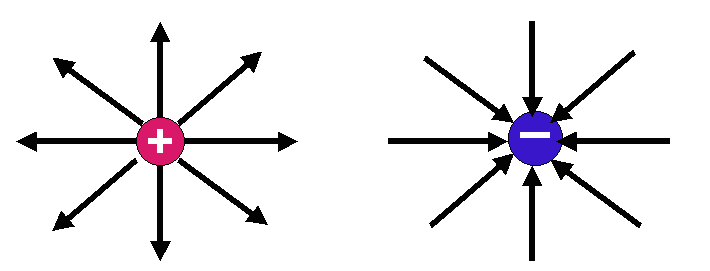
\includegraphics[width=0.60\textwidth]{./images/schematics/electric_field_lines_pos_and_neg_point_charges_1.png}\\
\end{center}

Gauss' law tells us, and it is easier to see that in its differential form, that
the {\bf electric charge is the source of the electric field}.

\end{frame}

% ------------------------------------------------------------------------------
% ------------------------------------------------------------------------------

%
% What to remember
%

\renewcommand{\lecturesummarytitle}{Main points to remember }
\renewcommand{\summarizedlecture}{2 }


%
%
%

\begin{frame}{Lecture \summarizedlecture - \lecturesummarytitle}

\begin{itemize}
{\small

\item {\bf Electric flux}
  \begin{itemize}
  {\small
     \item The electric flux $\Phi_E$ is the number of field lines of the electric field $\vec{E}$
           flowing through a surface S
        \begin{equation*}
          \Phi_E = \int_{S} \vec{E} d\vec{S}
        \end{equation*}
  }
  \end{itemize}

\item {\bf Gauss' law}
  \begin{itemize}
  {\small
     \item Our first Maxwell equation!
     \item In integral form (useful if a symmetry can be exploited to simplify the integral evaluation):
           Relates the flux through a closed surface with the net charge contained in it
           \begin{equation*}
              \int_{S} \vec{E} d\vec{S} = \frac{Q_{enc}}{\epsilon_0}
           \end{equation*}
     \item In differential form:
           Relates the divergence of the electric field with the local charge density
           \begin{equation*}
              \vec{\nabla} \vec{E} = \frac{\rho}{\epsilon_0}
           \end{equation*}
  }
  \end{itemize}

}
\end{itemize}

\end{frame}


%
% At the next lecture
%

\begin{frame}{At the next lecture (Lecture \nextlecture)}

\begin{itemize}
  \item {\bf Potential energy of a charge in an electrostatic field}
    \begin{itemize}
       \item we will generalise for discrete and continuous charge distributions
    \end{itemize}

  \vspace{0.4cm}
  \item {\bf Electric potential}

  \vspace{0.4cm}
  \item {\bf Circuital law for electrostatics} in differential and integral forms

  \vspace{0.4cm}
  \item Continue brushing up our relevant calculus skills

\end{itemize}

\end{frame}

%
% Optional reading
%

%
% Optional reading
%

\begin{frame}[plain,c]
\begin{center}
{\Huge \bf Optional reading for Lecture \thislecture}
\end{center}
\end{frame}

% ------------------------------------------------------------------------------

%
% Worked example :
%

{
\problemslide

\begin{frame}{Worked example: Exploiting the superposition principle}

  \begin{blockexmplque}{Question}
    A nonconductive solid sphere has a uniform volume charge density $\rho$.\\
    \vspace{0.1cm}
    Let $\vec{r}$ be the vector from the centre of the sphere to a general point
    $P$ within the sphere. As you should be able to easily confirm,
    the electric field $\vec{E}$ at a point $\vec{r}$  within the sphere is
    given by $\vec{E}(\vec{r}) = \rho \vec{r}/(3\epsilon_0)$.\\
    \vspace{0.1cm}
    If a spherical cavity is hollowed out of the sphere, as shown below,
    using superposition concepts, show that the electric field at all points
    within the cavity is uniform and equal to
    $\vec{E}(\vec{r})=\rho \vec{a}/(3\epsilon_0)$
    where $\vec{a}$ is the position vector
    from the centre of the sphere to the centre of the cavity.\\
    \begin{center}
      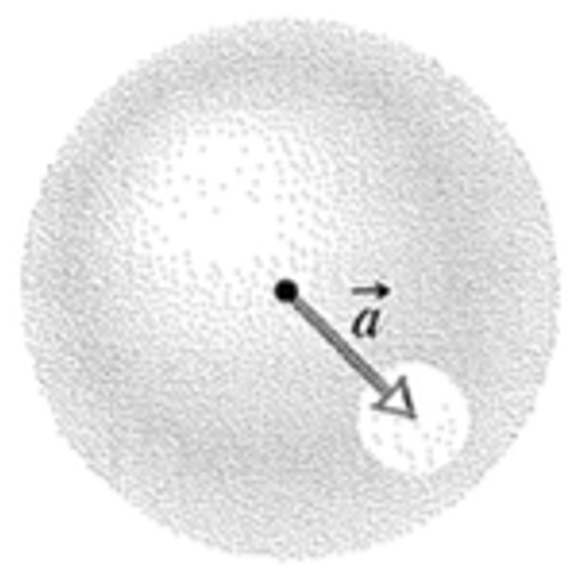
\includegraphics[width=0.20\textwidth]{./images/problems/lect02_spherical_charge_distribution_with_hole}
    \end{center}
  \end{blockexmplque}

\end{frame}

%
%
%

\begin{frame}{Worked example: Exploiting the superposition principle}

  The charge distribution in case of a uniformly charged solid sphere
  with a cavity is equivalent to that of
  a whole uniformly charged solid sphere of charge density $\rho$
  plus a smaller uniformly charged solid sphere
  of charge density -$\rho$ that fills the void.\\
  \vspace{0.2cm}

  \begin{columns}
    \begin{column}{0.38\textwidth}
      \begin{center}
        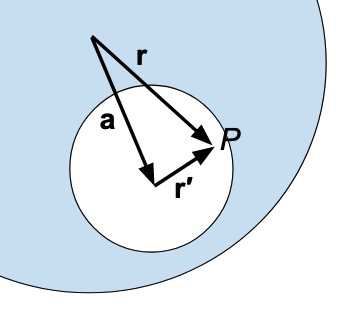
\includegraphics[width=0.95\textwidth]{./images/problems/lect02_sphere_with_cavity_distances_2}
      \end{center}
    \end{column}
    \begin{column}{0.62\textwidth}
      The field produced by each uniformly charged sphere is given.\\
      By superposition, the field at a point $P$ within the cavity
      (at distance $\vec{r}$ from the centre of the larger sphere)
      is given by
      \begin{equation*}
        \vec{E}(\vec{r}) =
        \frac{\rho \vec{r}}{3 \epsilon_0} +
        \frac{(-\rho) \vec{r}^\prime}{3 \epsilon_0} =
           \frac{\rho \vec{r}}{3 \epsilon_0} +
           \frac{(-\rho) (\vec{r} - \vec{a})}{3 \epsilon_0} \Rightarrow
      \end{equation*}
      \begin{equation*}
        \vec{E}(\vec{r}) =
           \frac{\rho \vec{a}}{3 \epsilon_0}
      \end{equation*}
    \end{column}
  \end{columns}

\end{frame}

} %\problemslide


% ------------------------------------------------------------------------------

%
% Worked example :
%

{
\problemslide

\begin{frame}{Worked example: Spherical shell with non-uniform density}

  \begin{blockexmplque}{Question}
    A spherical shell of inner radius $a$ and outer radius $b$ has volume charge
    density $\rho = kr^2$ ($a \le r \le b$), where $k$ is a constant and $r$ is
    the radial distance from the centre of the shell.\\
    Find the magnitude of the electric field $\vec{E}$
    produced by this charge distribution
    at radial distances i) $r<a$, ii) $a \le r < b$, and iii) $b \le r$.
  \end{blockexmplque}

  \vspace{0.2cm}

  Due to the obvious spherical symmetry, the electric field $\vec{E}$
  is a radial vector, and it is
  is going to be a function of only the radial distance $r$.\\

  \vspace{0.2cm}

  We have 3 distinct regions:
  i) $r<a$, ii) $a \le r < b$, and iii) $b \le r$.
  \vspace{0.2cm}

  For the calculation of $\vec{E}$ we will be applying Gauss's theorem:
  \begin{equation*}
    \int_{S} \vec{E} \cdot d\vec{S} =
      \frac{Q_{encl}}{\epsilon_0} =
        \frac{1}{\epsilon_0} \int_{\tau(S)} \rho d\tau
  \end{equation*}

\end{frame}

%
%
%

\begin{frame}{Worked example: Spherical shell with non-uniform density}

  For $r<a$, for {\em any possible} closed surface $S$
  that stays within that region of no charge, Gauss's theorem gives
  \begin{equation*}
    \int_{S} \vec{E} \cdot d\vec{S} = 0
  \end{equation*}
  Since this happens for all surfaces, it can not be the result of an
  accidental cancellation and it has to be that the integrand itself is 0.
  Therefore:
  \begin{equation}
    E (r<a) = 0
  \end{equation}

  \vspace{0.2cm}

  For $a \le r < b$, exploiting the spherical symmetry,
  we will be applying Gauss's theorem
  for a concentric spherical surface $S(r)$ of radius $r$.\\

  \vspace{0.2cm}

  Because both $\vec{E}$ and the surface vector $d\vec{S}$ are collinear,
  and the norm of $\vec{E}$ is constant, everywhere on $S(r)$,
  the flux calculation is simplified:
  \begin{equation*}
    \int_{S(r)} \vec{E} \cdot d\vec{S} =
    \int_{S(r)} E dS =
    E \int_{S(r)} dS =
    E 4\pi r^2
  \end{equation*}

\end{frame}

%
%
%

\begin{frame}{Worked example: Spherical shell with non-uniform density}

  The charge $Q_{enc}$, in the volume $\tau(S)$,
  enclosed by a spherical surface $S(r)$ of radius $r$
  is given by:
  \begin{equation*}
    Q_{enc} =
      \int_{\tau(S)} \rho d\tau =
      \int_{a}^{r} \Big( k u^2 \Big) 4\pi u^2 du =
      4\pi k \int_{a}^{r} u^4 du =
      \frac{4\pi k}{5} u^5 \Big\rvert_{a}^{r} \Rightarrow
  \end{equation*}
  \begin{equation*}
      Q_{enc} =
      \frac{4\pi k}{5} \Big(r^5 - a^5\Big)
  \end{equation*}

  Therefore, Gauss's law can be expressed as:
  \begin{equation*}
    E \cancel{4\pi} r^2 =
     \frac{\cancel{4\pi} k}{5 \epsilon_0} \Big(r^5 - a^5\Big)
  \end{equation*}

  This yields:
  \begin{equation*}
    E (a \le r < b)= \frac{k}{5 \epsilon_0} \Big(r^3 - \frac{a^5}{r^2}\Big)
  \end{equation*}

\end{frame}

%
%
%

\begin{frame}{Worked example: Spherical shell with non-uniform density}

  For $b \le r$, one can apply a similar analysis. In this case,
  $Q_{enc}$ is no longer a function of $r$
  since all spherical surfaces $S(r)$ include all charge.
  From the previous expression for $Q_{enc}$,
  setting $r$ equal to $b$, we have:
  \begin{equation*}
    Q_{enc} =
      \frac{4\pi k}{5} \Big(b^5 - a^5\Big)
  \end{equation*}

  Gauss's law can be expressed as:
  \begin{equation*}
    E \cancel{4\pi} r^2 =
     \frac{\cancel{4\pi} k}{5 \epsilon_0} \Big(b^5 - a^5\Big)
  \end{equation*}

  This yields:
  \begin{equation*}
    E (b \le r)= \frac{k}{5 \epsilon_0} \Big(\frac{b^5 - a^5}{r^2}\Big)
  \end{equation*}

  Summarizing, we found that:
  \begin{equation*}
    \displaystyle
    E =
      \begin{cases}
        0 & \text{ for } r < a\\
        \frac{k}{5 \epsilon_0} \Big(r^3 - \frac{a^5}{r^2}\Big) & \text{ for } a \le r < b\\
        \frac{k}{5 \epsilon_0} \Big(\frac{b^5 - a^5}{r^2}\Big) & \text{ for } b \le r
      \end{cases}
  \end{equation*}

\end{frame}

} %\problemslide

% ------------------------------------------------------------------------------

%
% Worked example :
% H/R Sec 23-9, problem 51 (page 626)
%

{
\problemslide

%
%
%

\begin{frame}{Worked example: Spherical shell and point charge}

  \begin{blockexmplque}{Question}
    The figure below shows
    a nonconducting spherical shell of
    inner radius $a$ and outer radius $b$.
    The shell has (within its thickness) a positive volume charge density
    $\rho(r)$ = $A/r$,
    where $A$ is a constant and $r$ is the distance from the center of the shell.
    In addition, a small ball of charge $q$ is located at that center.
    What value should A have if the electric field in the shell
    ($a < r < b$) is to be uniform?
    \begin{center}
      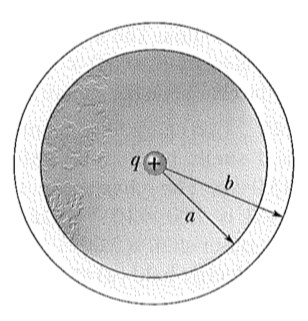
\includegraphics[width=0.30\textwidth]{./images/problems/lect02_thick_spherical_shell_and_central_charge}
    \end{center}
  \end{blockexmplque}

\end{frame}

%
%
%

\begin{frame}{Worked example: Spherical shell and point charge}

  Gauss's law in integral form is:
  \begin{equation*}
  	 \Phi = \frac{Q_{enc}}{\epsilon_0}
  \end{equation*}

  The electric flux $\Phi$ over a closed surface $S$ is defined as:
  \begin{equation*}
  	 \Phi = \oint_{S} \vec{E} \cdot d\vec{S}
  \end{equation*}

  Consider a spherical Gaussian surface with radius $r$, where $a < r < b$.
  Exploiting the spherical symmetry of the problem, we can write:
  \begin{equation*}
  	 \Phi = \oint_{S} E dS = E \oint_{S} dS = E 4\pi r^2
  \end{equation*}

\end{frame}

%
%
%

\begin{frame}{Worked example: Spherical shell and point charge}

  The charge in the volume $\tau(S)$,
  enclosed by the spherical Gaussian surface $S$ with radius $r$,
  is the charge $q$ at the origin and the fraction of the charge of the shell
  that is distributed at radial distances between $a$ and $r$.

  Therefore:
  \begin{equation*}
  	 Q_{enc} = q + \int_{\tau(S)}{\rho d\tau} \Rightarrow
  \end{equation*}

  \begin{equation*}
  	 Q_{enc} = q + \int_{a}^{r} \frac{A}{r^{\prime}} 4\pi {r^{\prime}}^{2} dr^{\prime} \Rightarrow
  	 Q_{enc} = q + 4\pi A \int_{a}^{r} r^{\prime} dr^{\prime} \Rightarrow
  \end{equation*}

  \begin{equation*}
  	 Q_{enc} = q + 4\pi A \frac{{r^{\prime}}^2}{2}\Big\rvert_{a}^{r} \Rightarrow
  	 Q_{enc} = q + 2\pi A (r^2 - a^2)
  \end{equation*}

  Combining the above exressions for $\Phi$ and $Q_{enc}$, we have:

  \begin{equation*}
  	 E 4\pi r^2 = \frac{1}{\epsilon_0} \Big( q + 2\pi A (r^2 - a^2) \Big)
  \end{equation*}

\end{frame}

%
%
%

\begin{frame}{Worked example: Spherical shell and point charge}

  Solving for $E$, we find:
  \begin{equation*}
  	 E = \frac{q + 2\pi A (r^2 - a^2)}{4\pi \epsilon_0 r^2} \Rightarrow
  	 E = \frac{1}{4\pi \epsilon_0 }
      \Big( \frac{q}{r^2} + 2\pi A - \frac{2\pi A a^2}{r^2} \Big)
  \end{equation*}

  The requirement that $E$ is uniform in the shell, implies that:
  \begin{equation*}
      \frac{q}{r^2} - \frac{2\pi A a^2}{r^2} = 0
  \end{equation*}

  Therefore:
  \begin{equation*}
      A = \frac{q}{2\pi a^2}
  \end{equation*}

\end{frame}

} %\problemslide

% ------------------------------------------------------------------------------

%
% Worked example :
% H/R, ch. 23, page 626, question 54
%

{
\problemslide

%
%
%

\begin{frame}{Worked example: Two uniformly charged spheres}

  \begin{blockexmplque}{Question}
    The figure below shows, in cross section, two solid spheres with uniformly
  	distributed charge throughout their volumes. Each has radius R.
  	Point P lies on a line connecting the centres of the spheres, at radial distance
  	R/2.00 from the centre of sphere 1.
  	If the net electric field at point P is zero, what is the ratio $q_2$/$q_1$
  	of the total charges?
    \begin{center}
      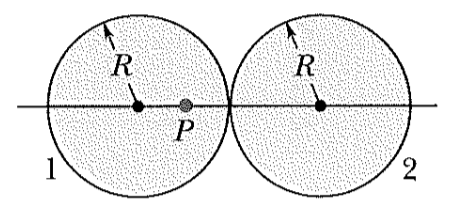
\includegraphics[width=0.60\textwidth]{./images/problems/lect02_2_charged_spheres}
    \end{center}
  \end{blockexmplque}

\end{frame}

%
%
%

\begin{frame}{Worked example: Two uniformly charged spheres}

  The electric field inside and outside a uniformly charged, nonconductive,
  solid sphere of radius $R$ was calculated earlier in this Lecture.\\
  \vspace{0.1cm}
  The results are summarised below:

  {\bf For $r < R$:}
  \begin{equation*}
     E(r) = \frac{Q \frac{r^3}{R^3}}{4 \pi \epsilon_0 r^2} =
      \frac{Q}{4 \pi \epsilon_0 R^3} r
  \end{equation*}

  {\bf For $r \ge R$:}
  \begin{equation*}
     E(r) = \frac{Q}{4 \pi \epsilon_0 r^2}
  \end{equation*}

  \vspace{0.1cm}

  The electric field $\vec{E}$ at point P is the superposition of 2 fields:
  the field $\vec{E}_1$ because of the presence of sphere 1 and
  the field $\vec{E}_2$ because of the presense of sphere 2:
  \begin{equation*}
  	 \vec{E}(P) = \vec{E}_1(P) + \vec{E}_2(P)
  \end{equation*}

\end{frame}

%
%
%

\begin{frame}{Worked example: Two uniformly charged spheres}

  Applying our previous result for the electric field:
  \begin{equation*}
  	\vec{E}_1(P) = \Big\{ \frac{Q}{4 \pi \epsilon_0 R^3} r \Big\} \hat{x} \xRightarrow{Q=q_1, \; r = R/2}
  	\vec{E}_1(P) = \Big\{ \frac{q_1/2}{4 \pi \epsilon_0 R^2} \Big\} \hat{x}
  \end{equation*}

  % \begin{equation*}
  % 	\vec{E}_1(P) = \Big\{ \frac{Q}{4 \pi \epsilon_0 R^3} r \Big\} \hat{x} \xRightarrow{Q=q_1, \; r = R/2}
  % 	\vec{E}_1(P) = \Big\{ \frac{q_1}{4 \pi \epsilon_0 R^3} \frac{R}{2} \Big\} \hat{x} \Rightarrow
  % \end{equation*}
  % \begin{equation*}
  % 	\vec{E}_1(P) = \Big\{ \frac{q_1/2}{4 \pi \epsilon_0 R^2} \Big\} \hat{x}
  % \end{equation*}

  and:
  \begin{equation*}
  	\vec{E}_2(P) = \Big\{ \frac{Q}{4 \pi \epsilon_0 r^2} \Big\} (-\hat{x}) \xRightarrow{Q=q_2, \; r = R+R/2 = 3R/2}
  	\vec{E}_2(P) = - \Big\{ \frac{4q_2/9}{4 \pi \epsilon_0 R^2} \Big\} \hat{x}
  \end{equation*}

  % \begin{equation*}
  % 	\vec{E}_2(P) = \Big\{ \frac{Q}{4 \pi \epsilon_0 r^2} \Big\} (-\hat{x}) \xRightarrow{Q=q_2, \; r = R+R/2 = 3R/2}
  % 	\vec{E}_2(P) = - \Big\{ \frac{q_2}{4 \pi \epsilon_0 (3R/2)^2} \Big\} \hat{x} \Rightarrow
  % \end{equation*}
  % \begin{equation*}
  % 	\vec{E}_2(P) = - \Big\{ \frac{4q_2/9}{4 \pi \epsilon_0 R^2} \Big\} \hat{x}
  % \end{equation*}

  Therefore, the total field is:
  \begin{equation*}
    \vec{E}(P) = \frac{1}{4 \pi \epsilon_0 R^2} (\frac{q_1}{2} - \frac{4q_2}{9}) \hat{x}
  \end{equation*}

  If E(P)=0, then:
  \begin{equation*}
  	\frac{q_1}{2} - \frac{4q_2}{9} = 0 \Rightarrow
    \frac{q_2}{q_1} = \frac{9}{8} \Rightarrow
  	\frac{q_2}{q_1} = 1.125
  \end{equation*}

\end{frame}


} %\problemslide

% ------------------------------------------------------------------------------


%
% Worked example :
% H/R Sec 23-9, problem 50 (page 625)
%

{
\problemslide

%
%
%

\begin{frame}{Worked example: Two spherical shells}

  \begin{blockexmplque}{Question}
    The figure on the left shows
    two nonconducting spherical shells fixed in place on an x axis.
    Shell 1 has uniform surface charge density +4.0 $\mu$C/m$^{2}$
    on its outer surface and radius 0.50 cm, and
    shell 2 has uniform surface charge density -2.0 $\mu$C/m$^{2}$
    on its outer surface and radius 2.0 cm. The shell centres are separated
    by a distance $L$ = 6.0 cm.
    Other than at $x = \infty$,
    where on the x axis is the net electric field equal to zero?
    \begin{center}
      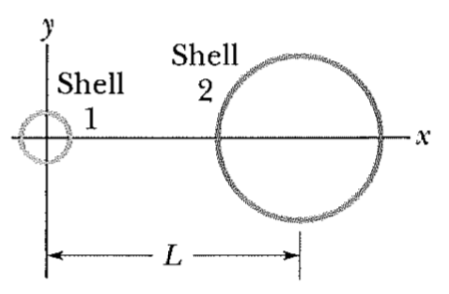
\includegraphics[width=0.40\textwidth]{./images/problems/lect02_2_charged_spherical_shells}
    \end{center}
  \end{blockexmplque}

\end{frame}

%
%
%

\begin{frame}{Worked example: Two spherical shells}

  Consider Gauss's law in its integral form:
  \begin{equation*}
  	 \oint_{S} \vec{E} \cdot d\vec{S} = \frac{Q_{enc}}{\epsilon_0}
  \end{equation*}
  Exploiting the symmetry of a system with charge $Q$ distributed
  uniformly on a spherical, nonconducting shell or radius $R$
  centred at the origin of the coordinate system,
  we can easily calculate the electric field:
  \begin{itemize}
  \item
  For $r < R$, the enclosed charge is 0 and from the symmetry of the problem we
  deduce that $\vec{E}(r) = 0$.
  \item
  For $r \ge R$, all charge Q is enclosed, and the electric field can
  be written (as if we had a point charge at the origin)
  as $\vec{E}(r) = \frac{Q}{4\pi\epsilon_0 r^2} \hat{r}$.\\
  \end{itemize}

  \vspace{0.2cm}
  The electric field $\vec{E}$ produced by the two spherical shells 1 and 2
  is given superposition principle:
  \begin{equation*}
    \vec{E} = \vec{E}_1 + \vec{E}_2
  \end{equation*}
  where $\vec{E}_1$ ($\vec{E}_2$) is the field of sphere 1 (2).\\

\end{frame}

%
%
%

\begin{frame}{Worked example: Two spherical shells}

  The field produced by each shell is pointing radially in (as in the case of
  the negatively charged shell 2) or out (as in the case of the positively
  charged shell 1). Therefore, for all points on the x axis,
  $\vec{E}_1$ and $\vec{E}_2$ point along $\pm \hat{x}$.\\

  \vspace{0.3cm}
  Within shell 1, $\vec{E}_1 = 0$, and within shell 2, $\vec{E}_2 = 0$.
  Therefore, within the shells, the net electric field $\vec{E}_1 + \vec{E}_2$
  cannot be zero there.\\

  \vspace{0.3cm}

  For all x values between the shells ($R_1 < x < L-R_2$),
  the fields $\vec{E}_1$ and $\vec{E}_2$ point in the same direction
  and, therefore, the net electric field $\vec{E}_1 + \vec{E}_2$
  cannot be zero there.\\

  \vspace{0.3cm}

  The charge contained by shells 1 and 2 can be calculated as follows:

  \begin{equation*}
  	 Q_1 = 4\pi R_{1}^{2} \sigma_{1}
         = 4\pi (5\times 10^{-3} \; m)^{2} (4 \times 10^{-6} \; C/m^2)
         = 4\pi \times 10^{-10} \; C
  \end{equation*}
  \begin{equation*}
  	|Q_2| = 4\pi R_{2}^{2} |\sigma_{2}|
          = 4\pi (2\times 10^{-2} \; m)^{2} (2 \times 10^{-6} \; C/m^2)
          = 8 \times 4\pi \times 10^{-10} \; C
  \end{equation*}

\end{frame}

%
%
%

\begin{frame}{Worked example: Two spherical shells}

  Since $|Q_2| > Q_1$,
  $|\vec{E}_2|>|\vec{E}_1|$ for all values of $x > L + R_2$
  (closer to shell 2 than to shell 1). Therefore,
  the net field $\vec{E}_1 + \vec{E}_2$ cannot be zero there.\\

  \vspace{0.3cm}

  Following from the above, the only range of x values where
  the net field $\vec{E}_1 + \vec{E}_2$ can be zero, is $x < -R_1$.
  In that range,  $\vec{E}_1$ and $\vec{E}_2$ have opposite directions,
  and magnitudes given by:

  \begin{equation*}
  	 E_1 = \frac{1}{4\pi \epsilon_0} \frac{Q_1}{|x|^2} \xRightarrow{4\pi R_{1}^{2} \sigma_{1}}
  	 E_1 = \frac{R_{1}^{2} \sigma_{1}}{\epsilon_0} \frac{1}{|x|^2}
  \end{equation*}

  \begin{equation*}
  	 E_2 = \frac{1}{4\pi \epsilon_0} \frac{|Q_2|}{(L+|x|)^2} \xRightarrow{|Q_2|=4\pi R_{2}^{2} |\sigma_{2}|}
  	 E_2 = \frac{R_{2}^{2} |\sigma_{2}|}{\epsilon_0} \frac{1}{(L+|x|)^2}
  \end{equation*}

  The requirement that the net electric field is zero, implies that:
  \begin{equation*}
  	 E_1 = E_2
  \end{equation*}

\end{frame}

%
%
%

\begin{frame}{Worked example: Two spherical shells}

  Therefore:
  \begin{equation*}
    \frac{R_{1}^{2} \sigma_{1}}{\epsilon_0} \frac{1}{|x|^2} =
    \frac{R_{2}^{2} |\sigma_{2}|}{\epsilon_0} \frac{1}{(L+|x|)^2} \Rightarrow
  \end{equation*}

  \begin{equation*}
    \Big( \frac{L+|x|}{|x|} \Big)^2 = \frac{R_{2}^{2} |\sigma_{2}|}{R_{1}^{2} \sigma_{1}} \Rightarrow
    \frac{L}{|x|} + 1  = \frac{R_{2}}{R_{1}} \sqrt{\frac{|\sigma_{2}|}{\sigma_{1}}} \Rightarrow
  \end{equation*}

  \begin{equation*}
    |x| = \frac{L}{ \frac{R_{2}}{R_{1}} \sqrt{\frac{|\sigma_{2}|}{\sigma_{1}}} - 1} \Rightarrow
  \end{equation*}

  \begin{equation*}
    |x| = \frac{6\; cm}{ \frac{2.0}{0.5} \sqrt{\frac{2}{4}} - 1}
        = \frac{6\; cm}{ \frac{4}{\sqrt{2}} - 1} \approx 3.28 \; cm
    \Rightarrow
    x \approx -3.28 \; cm
  \end{equation*}

\end{frame}

} %\problemslide

% ------------------------------------------------------------------------------

%
% Worked example :
%

{
\problemslide

\begin{frame}{Worked example: Electric field of two charged sheets}

  \begin{blockexmplque}{Question}
       Two uniform infinite sheets of electric charge densities
       $+\sigma$ and $-\sigma$ intersect at a right angle.
       Find the magnitude and direction of the electric field everywhere
       and sketch the electric field lines.
  \end{blockexmplque}

  The magnitude of the electric field caused by a single, infinite sheet
  of uniform charge density $\sigma$ is given by:
  \begin{equation*}
     E = \frac{\sigma}{2\epsilon_0}
  \end{equation*}

  The direction of the field is perpendicular to the sheet and it is pointing
  towards (away from) the sheet, if it is negatively (positively) charged.

  The field in the problem of two uniform infinite sheets
  can be obtained by invoking the superposition principle
  and superimposing undisturbed
  \begin{itemize}
  \item
  the field $\vec{E_(+)}$
  of an infinite sheet of uniform charge density $+\sigma$, and
  \item
  the field $\vec{E_(-)}$
  of an infinite sheet of uniform charge density $-\sigma$.
  \end{itemize}

\end{frame}

%
%
%

\begin{frame}{Worked example: Electric field of two charged sheets}

  The magnitude of the combined field ($\vec{E}$) is:
  \begin{equation*}
     E = \sqrt{E_(+)^2 + E_(-)^2}
       = \sqrt{\Big( \frac{+\sigma}{2\epsilon_0} \Big)^2 +
               \Big( \frac{-\sigma}{2\epsilon_0} \Big)^2} \Rightarrow
     E = \frac{\sqrt{2}\sigma}{2\epsilon_0}
  \end{equation*}
  The field lines are sketched below:
  \begin{figure}[htb]
    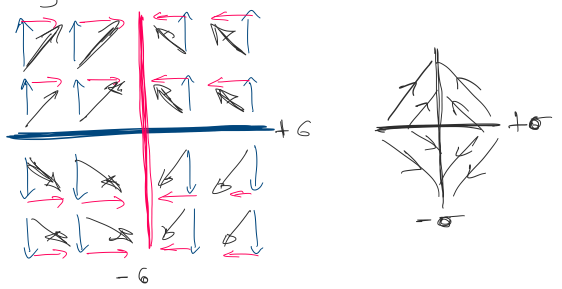
\includegraphics[width=0.8\linewidth]{./images/problems/lect02_field_lines_of_2_charged_sheets}
  \end{figure}


\end{frame}

} %\problemslide

% ------------------------------------------------------------------------------

{
\programmingslide

%
%
%

\begin{frame}{PHYS201 scientific programming task for Lecture \thislecture}

{\small

If you did the previous task, you already have a program to calculate the
electric field (in 2-D) for an arbitrary distribution of discrete charges.\\
\vspace{0.2cm}

Generalize your previous program:
\begin{itemize}
{
  \item Move from a 2-D to a {\bf 3-D calculation}.
  \item Add an option to {\bf specify a continuous distribution of charge}
        (i.e. work with a user-defined charge density function $\rho(\vec{r})$)
}
\end{itemize}

\vspace{0.2cm}
What you will be doing, is to perform the following numerical integration:
\begin{equation*}
   \vec{E}(\vec{r}) = \frac{1}{4\pi\epsilon_0} \int_{\tau}
      d\tau^{\prime} \frac{\rho({\pvec{r}'})}{|\vec{r}-\pvec{r}'|^{3}} (\vec{r}-\pvec{r}')
\end{equation*}

\vspace{0.3cm}

Can you test Gauss' law numerically?

}
\end{frame}

%
%
%

\begin{frame}{PHYS201 scientific programming task for Lecture \thislecture}

{\small

As an example, use the following charge density in spherical coordinates:
\begin{equation*}
   \rho =
     \begin{cases}
       \frac{\rho_0}{(r/r_0)^2} e^{-r/r_0} cos^2\phi, & \text{if $r < 5 r_0$} \\
       & \\
       0, \text{otherwise}
     \end{cases}
\end{equation*}
where $\rho_0$ = 0.16 C/m$^{3}$ and r$_0$ = 10 cm.\\
%
% at r = 5 *r0, the charge contained is 6.24 * \rho_0 * ro^3
% 0.16 is 1/6.24
%

\vspace{0.2cm}
Calculate numerically the amount of charge Q enclosed in a sphere of radius r, as a function or r:\\
\begin{equation*}
  Q(r) = \int_{0}^{r} \int_{4\pi} d\tau \rho(\vec{r^\prime})
\end{equation*}

\vspace{0.2cm}
Confirm that your distribution plateaus to a value of $Q_{tot}$ for
r $>5r_0$, as the sphere encloses all regions of non-zero charge density.
What is the value of $Q_{tot}$?\\

\vspace{0.2cm}
Calculate the electric flux through the surface of a sphere with radius r = 5$r_0$
and confirm that:
\begin{equation*}
  \epsilon_0 \oint \vec{E} \cdot d\vec{S} = Q_{tot}
\end{equation*}
}

\end{frame}

} % programming

